%%%%%%%%%%%%%%%%%%%%%%%%%%%%%%%%%%%%%%%%%%%%%%%%%%%%%%%%%%%%%%%%%%%%%%%%
%    INSTITUTE OF PHYSICS PUBLISHING                                   %
%                                                                      %
%   `Preparing an article for publication in an Institute of Physics   %
%    Publishing journal using LaTeX'                                   %
%                                                                      %
%    LaTeX source code `ioplau2e.tex' used to generate `author         %
%    guidelines', the documentation explaining and demonstrating use   %
%    of the Institute of Physics Publishing LaTeX preprint files       %
%    `iopart.cls, iopart12.clo and iopart10.clo'.                      %
%                                                                      %
%    `ioplau2e.tex' itself uses LaTeX with `iopart.cls'                %
%                                                                      %
%%%%%%%%%%%%%%%%%%%%%%%%%%%%%%%%%%
%
%
% First we have a character check
%
% ! exclamation mark    " double quote  
% # hash                ` opening quote (grave)
% & ampersand           ' closing quote (acute)
% $ dollar              % percent       
% ( open parenthesis    ) close paren.  
% - hyphen              = equals sign
% | vertical bar        ~ tilde         
% @ at sign             _ underscore
% { open curly brace    } close curly   
% [ open square         ] close square bracket
% + plus sign           ; semi-colon    
% * asterisk            : colon
% < open angle bracket  > close angle   
% , comma               . full stop
% ? question mark       / forward slash 
% \ backslash           ^ circumflex
%
% ABCDEFGHIJKLMNOPQRSTUVWXYZ 
% abcdefghijklmnopqrstuvwxyz 
% 1234567890
%
%%%%%%%%%%%%%%%%%%%%%%%%%%%%%%%%%%%%%%%%%%%%%%%%%%%%%%%%%%%%%%%%%%%
%

%AIP Reprint Class%%%%%%%%%%%%%%%%%%%%%%%%%%%%%%%%%%%%%%%%%%%%%%%%%%%%%%%%%%%%%%%%%%%%%%%%%%%%%
\documentclass[aip,prl,amsmath,amssymb,reprint,superscriptaddress]{revtex4-1} %preprint version
\usepackage{graphicx}% Include figure files
\usepackage{dcolumn}% Align table columns on decimal point
\usepackage{bm}% bold math
\usepackage{epstopdf}

    \renewcommand{\topfraction}{0.9}    % max fraction of floats at top
    \renewcommand{\bottomfraction}{0.8}    % max fraction of floats at bottom
    \setcounter{topnumber}{2}
    \setcounter{bottomnumber}{2}
    \setcounter{totalnumber}{4}     % 2 may work better
    \setcounter{dbltopnumber}{2}    % for 2-column pages
    \renewcommand{\dbltopfraction}{0.9}    % fit big float above 2-col. text
    \renewcommand{\textfraction}{0.07}    % allow minimal text w. figs
    \renewcommand{\floatpagefraction}{0.7}    % require fuller float pages
    \renewcommand{\dblfloatpagefraction}{0.7}    % require fuller float pages
    \setlength{\abovecaptionskip}{5pt}
    \setlength{\belowcaptionskip}{5pt}
    \setlength{\parskip}{0pt}
    \setlength{\textfloatsep}{5pt} 

%%%%%%%%%%%%%%%%%%%%%%%%%%%%%%%%%%%%%%%%%%%%%%%%%%%%%%%%%%%%%%%%%%%%%%%%%%%%%%%%%%%%%%%%%%%%%%%%%%

%IOP preprint class %%%%%%%%%%%%%%%%%%%%%%%%%%%%%%%%%%%%%%%%%%%%%%%%%%%%%%%%%%%%%%%%%%%%%%%%%%%%%%
%\documentclass[12pt]{iopart}
%\newcommand{\gguide}{{\it Preparing graphics for IOP journals}}
%Uncomment next line if AMS fonts required
%\usepackage{iopams}
%\usepackage{graphicx}
%\usepackage{epstopdf}  
%%%%%%%%%%%%%%%%%%%%%%%%%%%%%%%%%%%%%%%%%%%%%%%%%%%%%%%%%%%%%%%%%%%%%%%%%%%%%%%%%%%%%%%%%%%%%%%%%%
%Slava's inserts %%%%%%%%%%%%%%%%%%%%%%%%%%%%%%%%%%%%%%%%%%%%%%%%%%%%%%%%%%%%%%%%%%%%%%%%%%%%%%
%\usepackage{amsfonts}
%\usepackage{amssymb}

%\newcommand{\ptt}[1]{\frac{\partial#1}{\partial t}}
%\newcommand{\vvec}{\mathbf{v}}
%\newcommand{\Bvec}{\mathbf{B}}
%\newcommand{\Evec}{\mathbf{E}}
%\newcommand{\Jvec}{\mathbf{J}}
%\newcommand{\Avec}{\mathbf{A}}
%%%%%%%%%%%%%%%%%%%%%%%%%%%%%%%%%%%%%%%%%%%%%%%%%%%%%%%%%%%%%%%%%%%%%%%%%%%%%%%%%%%%%%%%%%%%%%%%%%

\begin{document}
\title{Turbulence Analysis of an MHD wind-tunnel plasma: Spectral comparisons and observation of variance anisotropy}

\author{D.A. Schaffner}
\affiliation{Swarthmore College, Swarthmore, PA, USA}
\author{M.R. Brown}
\affiliation{Swarthmore College, Swarthmore, PA, USA}
\author{V.S. Lukin}
\affiliation{Space Science Division, Naval Research Laboratory, Washington, DC, USA}

\date{\today}
\begin{abstract}
Variance anisotropy observed in magnetic fluctuations on the Swarthmore Spheromak Experiment (SSX).
\end{abstract}

\maketitle

\section{Introduction}

The solar wind turbulence community has seen a flurry of results in recent years, as diagnostic capabilities on spacecraft have steadily improved, especially in the temporal resolution which has allowed for investigation into ion, sub-ion and electron scale turbulence measurements. In addition, newer analysis techniques have been developed to better tap the details of the rich turbulent environment that is the heliosphere. 

Analysis of timeseries fluctuations in the guise of spectrum analysis has served as the foundation for turbulence research in the solar wind~\cite{goldstein95,tumarsch95}. Improving diagnostics has led to ever greater precision in measurements of spectral indices for both magnetic and velocity fluctuation spectra~\cite{podesta07}, as well as increasing resolution of scale, allowing for measurements of spectra of sub-ion and electron scale fluctuations~\cite{alexandrova09,sahraoui09}. However, many outstanding questions regarding the nature of this turbulence, including both injection and dissipation mechanisms, have prompted research beyond typical spectral analysis. Two such avenues have been the exploration of the anisotropic nature of the turbulence and comparison of spectra between different observables (i.e. magnetic versus density fluctuations).

Theoretical treatments of magnetized plasma turbulence have almost universally predicted anisotropy to develop based on directions perpendicular and parallel to a mean field vector; many forms of this anisotropy has been predicted and observed (a good overview of the various types is given in Horbury 2012)~\cite{horbury12}. This paper focuses on variance anisotropy---the observation of greater magnetic fluctuation power in components perpendicular to the mean magnetic field versus parallel. From the experimentalist point of view, this is the most straightforward quantity to report and a reasonable place to begin. Analysis of other forms of anisotropy are saved for future work.---%has garnered great interest as it is viewed as a keystone result for theoretical understanding of MHD turbulence. 

Anisotropy is a common theme in solar wind turbulence and is predicted to be present by many turbulence theories. Since the solar wind speeds are typically super-Alfvenic, anisotropy studies generally reference the velocity vector of the bulk flow when defining perpendicular versus parallel fluctuations. Variance anisotropy, however, references a mean magnetic field vector---either global or local mean.

Comparison amongst fluctuation spectra (typically magnetic, flow, and density fluctuations) also provide insight into the nature of the turbulence. For example, relative partition of fluctuation energy between magnetic and kinetic can be useful in making determinations of turbulent properties~\cite{podesta07} or comparison of the spectral indices of magnetic and density spectra suggest an increase in the compressibility of a plasma(the so-called density bulge~\cite{harmon05}). Comparison of velocity and magnetic spectra at injection scales can also be used to hypothesis on the generating mechanisms of the turbulence~\cite{}(cite needed).

As results from space become more detailed, comparison to simulation and laboratory experiment become more useful in order to better develop the theory as well as inform future space missions. Much progress has been made to develop laboratory experiment which can inform space plasma research~\cite{howes12a} as well as begin to make turbulence measurements~\cite{ren11}.  Experiments conducted in the MHD wind-tunnel configuration of the Swarthmore Spheromak Experiment have shown the ability to produce and analyze MHD turbulence using many of the same methods used in the space plasma community, and has produced turbulence measurements which are comparable to \textit{in-situ} results~\cite{schaffner14a}. Moreover, using varying amounts of helicity injection, some characteristics of the turbulence can be modified~\cite{schaffner14b}.

A full spectral analysis of fluctuations in the SSX has been conducted, including magnetic field, density and Mach flow fluctuations. Using a wavelet transform method to decompose the timeseries signal, the magnetic field fluctuation spectra can be broken into portions that are parallel or perpendicular to the local magnetic field vector. Analysis of these portions show that parallel fluctuation power decreases slightly faster than that for perpendicular fluctuations generating a separating in power as a function of increasing frequency. This effect in frequency space is very close to the observation of variance anisotropy seen in wavenumber space in solar wind turbulence~\cite{kiyani13}. The ratio is shown to grow from nearly isotropic levels in the energy injection scale to a maximum $\perp/\parallel$ ratio of 3 at frequencies of about 1MHz. Beyond this point, the ratio begins to contract reaching isotropy around 10MHz. Though the axial flow speeds of the plasma in the wind-tunnel sub-Mach, if a Taylor hypothesis were still invoked this peak in the ratio would correspond to the ion inertial scale length. 

Since density and mach fluctuations timeseries are also recorded, comparisons amongst these spectra are also reported. Comparison of Mach number fluctuation spectra (as a proxy for flow) to magnetic spectra in the lowest frequencies suggests that energy injection into the turbulent spectra is primarily magnetic. This result is consistent with the nature of the spheromak generation process. Also the indices of density and magnetic spectra appear to diverge at a scale consistent with the ion inertial length and also where anisotropy is found to decrease. Both results would be consistent with an increase in compressibility of the plasma due to ion scale physics. However, firm conclusions are not made as noise issues in the density and flow diagnostics at that scale may be a factor.

The organization of this paper is as follows: First, a brief description of the plasma laboratory is given. Then, an overview of the analysis techniques used to determine perpendicular and parallel fluctuations is provided; details of the method and a second method used to verify its validity are described in the appendix. The results of this analysis is provided in section 4 including how spectra scaling varies with helicity injection, and how it evolves in time. In section 5 a comparison of magnetic fluctuation spectra is made to velocity and density fluctuations as well. Section 6 gives a discussion of how all of these spectra results are consistent with the observation of an ion inertial scale in the plasma. Comparison to a MHD simulation is made in section 7 and conclusions are presented in section 8.

\section{Experiment}

A turbulence cascade process in a laboratory experiment is naturally going to have a different origin than a space physics process; however, it is assumed that processes after the energy injection state (i.e. energy transfer in the inertial range and dissipation) will be similar enough so that exploration of the physics behind them in the laboratory can be beneficial to an overall understanding.

\begin{figure}[!htbp]
\centerline{
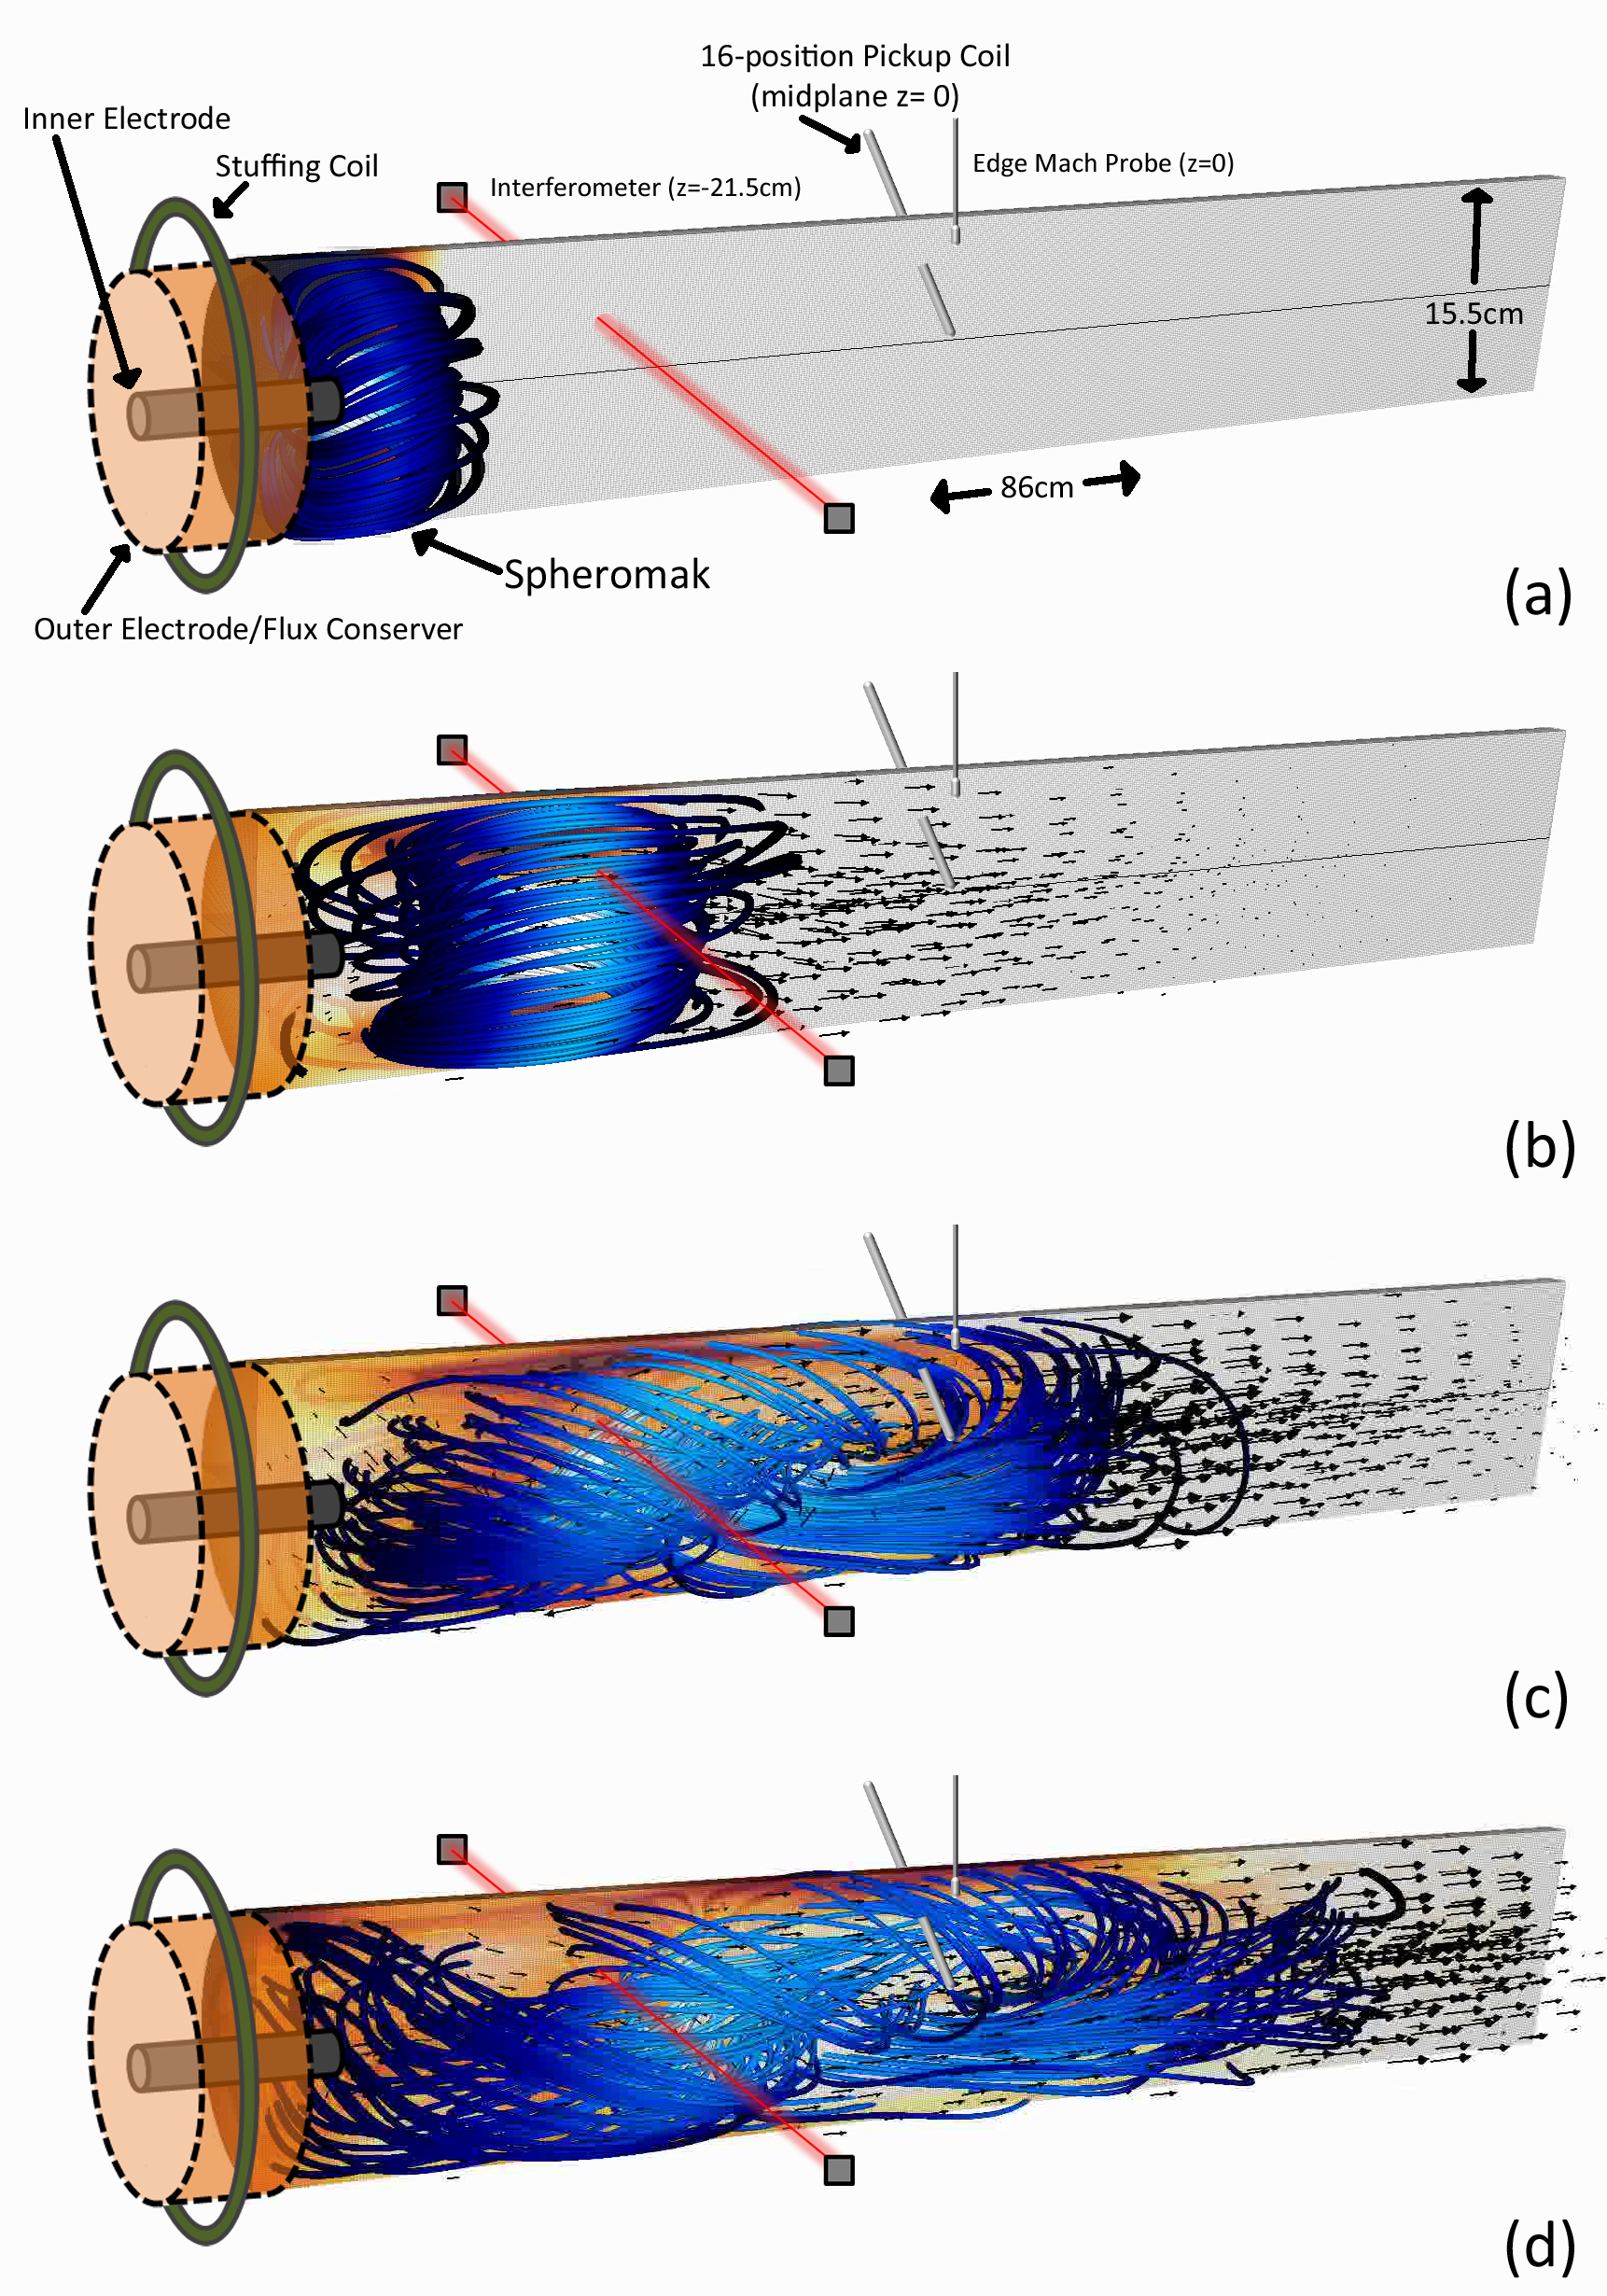
\includegraphics[width=8.5cm]{simulation_diagram_4panel.eps}}
\caption{\label{fig:moviestills}}
\end{figure}

The energy for the turbulence found in the MHD wind-tunnel in the Swarthmore Spheromak Experiment originates in the plasma production process. A plasma gun configuration sits on one end of the 15.5cm diameter, 86cm long cylindrical copper column which constitutes the MHD wind-tunnel. The gun consists of a tungsten-coated 4cm wide inner electrode placed concentrically within the copper cylinder which serves as an outer electrode. An axial aligned wire coil surrounds both electrodes and current is supplied to the coil to produce a known amount of magnetic flux---between 0 and 1.5mWb---axially through the inner electrode---this flux is referred to as stuffing flux, $\Phi$. A 1mF capacitor bank, charged to 4kV is discharged across the electrodes; this voltage fully ionizes a small volume of hydrogen gas puffed in just before the discharge. Radial currents through this newly produced plasma push the plasma down the column and into the fringe magnetic fields which tend to resist this push and stuff the progress of the plasma (hence the term, stuffing flux). Given enough current, and thus large enough $J\times B$ force, the plasma distends the stuffing fields until they break off, forming a self-contained magnetic field structure called a spheromak. This structure is visualized in Figure~\ref{fig:moviestills}(a) extracted from a simulation. Since the spheromak has both polodial and torodial magnetic fields, the relative ratio of field strength between these two directions is quantified by the magnetic helicity, defined as,
\begin{equation}
K_{B} = \int A \cdot B dV
\label{eq:helicity_th}
\end{equation}
where A is the vector potential and dV is the volume element. Previous work has shown that magnetic helicity of the plasma scales approximately linearly with the amount of stuffing flux applied to the gun~\cite{schaffner14b}

The generalized turbulence cascade begins with this compact magnetic structure. Inside the wind-tunnel, the magnetic structure is energetically unstable---the structure will begin to tilt over and expand into the remainder of the wind-tunnel. Because the column is copper, and thus flux conserving, the magnetic helicity is conserved unlike the magnetic energy. The structure then also begins to twist as it tilts over. The free energy released in the fall-over materializes as fluctuations in the field, generating the turbulent cascade. Figures~\ref{fig:moviestills}(a-d) show a generalized version of this process through simulation. The turbulent fluctuations are most prominent in the fourth panel. In the actual experiment, the gun typically injects more than a single, self-contained structure so while an initial structure is decaying, more compact field energy is being injected. This allows for a time frame of stationary fluctuations that is used in the turbulence analysis.

The turbulence data is extracted from magnetic, density and flow measurements during this stationary period. Magnetic fluctuations are recorded using 3mm wide, single loop pick-up coils located at 16 radial locations along the radius of the midplane of the column. Each radial position has three orthogonal loops oriented along the axial, radial and azimuthal directions of the column. A 64MHz, 14-bit DTaq digitizer records $dB/dt = \dot{B}$ timeseries data which is converted into magnetic fluctuation data in frequency space (as discussed in the following section). Line-integrated density data is measured with a HeNe interferometer located 21.5cm off of the midplane and flow fluctuations are estimated from a Mach probe located on the edge of the copper column at the midplane (as indicated in Figure~\ref{fig:moviestills}(a)). Bulk flow of the plasma is estimated with time-of-flight measurements between the density signal at z=-21.5cm and the magnetic signal at the midplane, z=0. The plasma is also generated with a set amount of magnetic helicity which is governed by initial conditions of the plasma gun source---namely, amount of flux generated in the gun core (called stuffing flux). The helicity can be scanned~\cite{schaffner14b}, but in this work focus is primarily on two states: a state with non-zero helicity labeled by the amount of core flux (1.0mWb) and a state with no injected helicity (0.0mWb). Table~\ref{tab:params} indicates typical plasma parameter values for these two states.

Each dischrage of the plasma gun constitutes an experimental shot and typically lasts for about 120$\mu s$ from formation of the magnetic fields to their eventual resistive dissipation. The turbulence data reported here is extracted from a time range of 40 to 60$\mu s$. This is the epoch during each shot where the fluctuations are most stationary; energy at the probe location is balanced between injection energy from the gun and loss through advection away from the probe and through possible dissipation mechanisms (including resistive decay of the currents).

An ensemble average for each helicity state is constructed from 40 shots.

\section{Analysis Techniques}\label{sec:analysis}

The bulk of the data of this paper is analyzed in frequency space using either a Wavelet transform method~\cite{torrence98} or a traditional Fast-Fourier Transform (FFT). Timeseries data transformed using a sixth-order Morlet mother wavelet with 256 logarithm scale steps per octave. For magnetic fluctuations, the wavelet transform is applied directly to the $\dot{B}(t)$ data from the pickup coils, separately for each orthogonal component, $x$. Each shot contains 8192 timesteps and the transform is applied to the entire shot to yield an $W_{x}(f,t)$. A known conversion factor is applied transform the wavelet scales into Fourier frequencies. Then, the transform is summed over the time range of interest, typically 40-60$\mu s$. Then, the transforms are divided through by the square of the frequency to yield,
\begin{equation}
B_{x}(f) = \frac{1}{f^{2}}\sum_{t=t_{0}}^{t_{1}} W_{x}(f,t)
\label{eq:wavelet_transform}
\end{equation}.

Since the entire shot is being used in the wavelet transform, the frequency range can extend beyond that which would be typical the time range under analysis. The entire frequency range is displayed in the following plots, but the focus of the analysis will be on the same frequency range accessible by an FFT.

A similar procedure is applied to the density timeseries from the interferometer and the Mach number timeseries from the Mach probe, but without the frequency scaling used for the magnetic.

For spatial spectra (using separate radial points on the magnetics probe) an FFT is used.

The method for conversion of the magnetic fluctuation spectra from $\vec{B} = (B_{r},B_{\theta},B_{z})$ to $\vec{B} = (B_{\parallel},B_{\perp}$) for the variance anisotropy analysis is detailed in the appendix.

\section{Variance Anisotropy}\label{sec:variance}

\begin{figure}[!htbp]
\centerline{
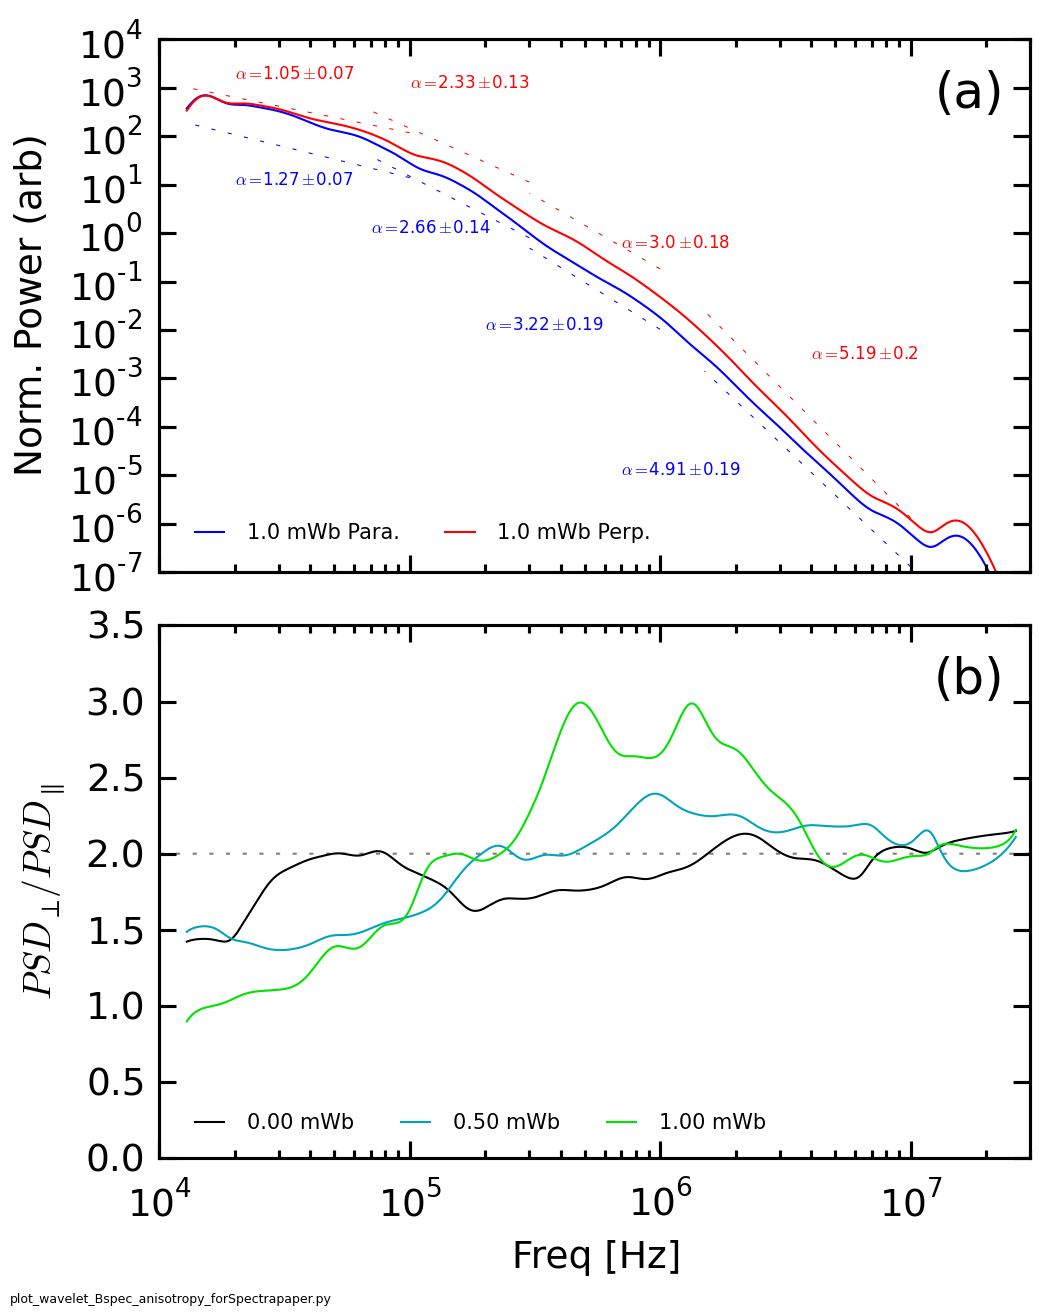
\includegraphics[width=8.5cm]{Bperppara_chan1t4_1mWbspectra_40t60us_wAsymRatio}}
\caption{\label{fig:spectra}}
\end{figure}

The magnetic field fluctuation spectra perpendicular and parallel to the local magnetic field vector is shown in figure~\ref{fig:spectra}(a) averaged over 40 shots and the inner four probe tips. Like previously reported magnetic spectra~\cite{schaffner14a}, both perpendicular and parallel curves exhibit power-law like behavior for most frequencies between 10kHz and 10MHz. Fits can be made to various sections of the curve using a Maximum Likelihood Estimation method~\cite{clauset09}; the short fits show that the scaling appears to gradually change from spectral indices of about 1 in the injection (or outer) range and from about 2.5 to 5 in the remaining sections. As has been noted before, with the exception of the injection range slope, the inertial and possibly dissipation range spectral indices are steeper than observed in solar wind turbulence spectra.

However, the separation between perpendicular and parallel spectra proceed in a manner similar to that found in space. Both perpendicular fluctuations (red) and parallel fluctuations (blue) begin at roughly the same magnitude in power. Beyond 20kHz, though, the parallel curve dips down slightly faster than the perpendicular and this trend continues up to about 500kHz. Then the separation begins to decrease and approaches a constant value from 5MHz to the Nyquist limit of 32MHz. This gradual change as a function of frequency is more clearly observed in figure ~\ref{fig:spectra}(b) plotted in log-linear format, which provides the ratio of the two curves in figure~\ref{fig:spectra}(a). Since the fluctuations perpendicular to the B-field have two component directions while parallel fluctuations have only one, the point of isotropy, or equal fluctuations in all three components) occurs when the ratio of perpendicular to parallel equal to 2. Isotropy is indicated in figure~\ref{fig:spectra}(b) by the dashed gray line.

At the lowest frequencies, the balance of power actually tips toward parallel over perpendicular. As the frequency decreases, an thus, presumably, the scale size decreases, the ratio approaches isotropy, then changes over to a dominantly perpendicular power level. The ratio continues to steadily increase reaching a peak of about 3 at about 500kHz. There is a brief dip before the ratio rises again at about 1.5MHz; at this point, the ratio begins to drop steadily, and approaches an isotropic level at about 5MHz. 

The scale dependency of the 1.0mWb data can be compared to other helicity levels. The black curve shows the anisotropy ratio for the zero helicity state, when the field strength is about an order of magnitude less, and there is much less structure to the field. As might be expected for such a state, there appear to be very little anisotropy at any scale with values staying close to R=2. The blue curve, showing the anisotropy ratio for a 0.5mWb stuffing case, clearly shows intermediate ratios between the 1.0 and 0.0mWb plasmas. This observation is somewhat curious as there is very little difference in magnetic field magnitude between 1.0mWb and 0.5mWb; the only difference between to the two states is the amount of average flow (which would not be expected to affect anisotropy) and the amount of helicity in the plasma.

\begin{figure}[!htbp]
\centerline{
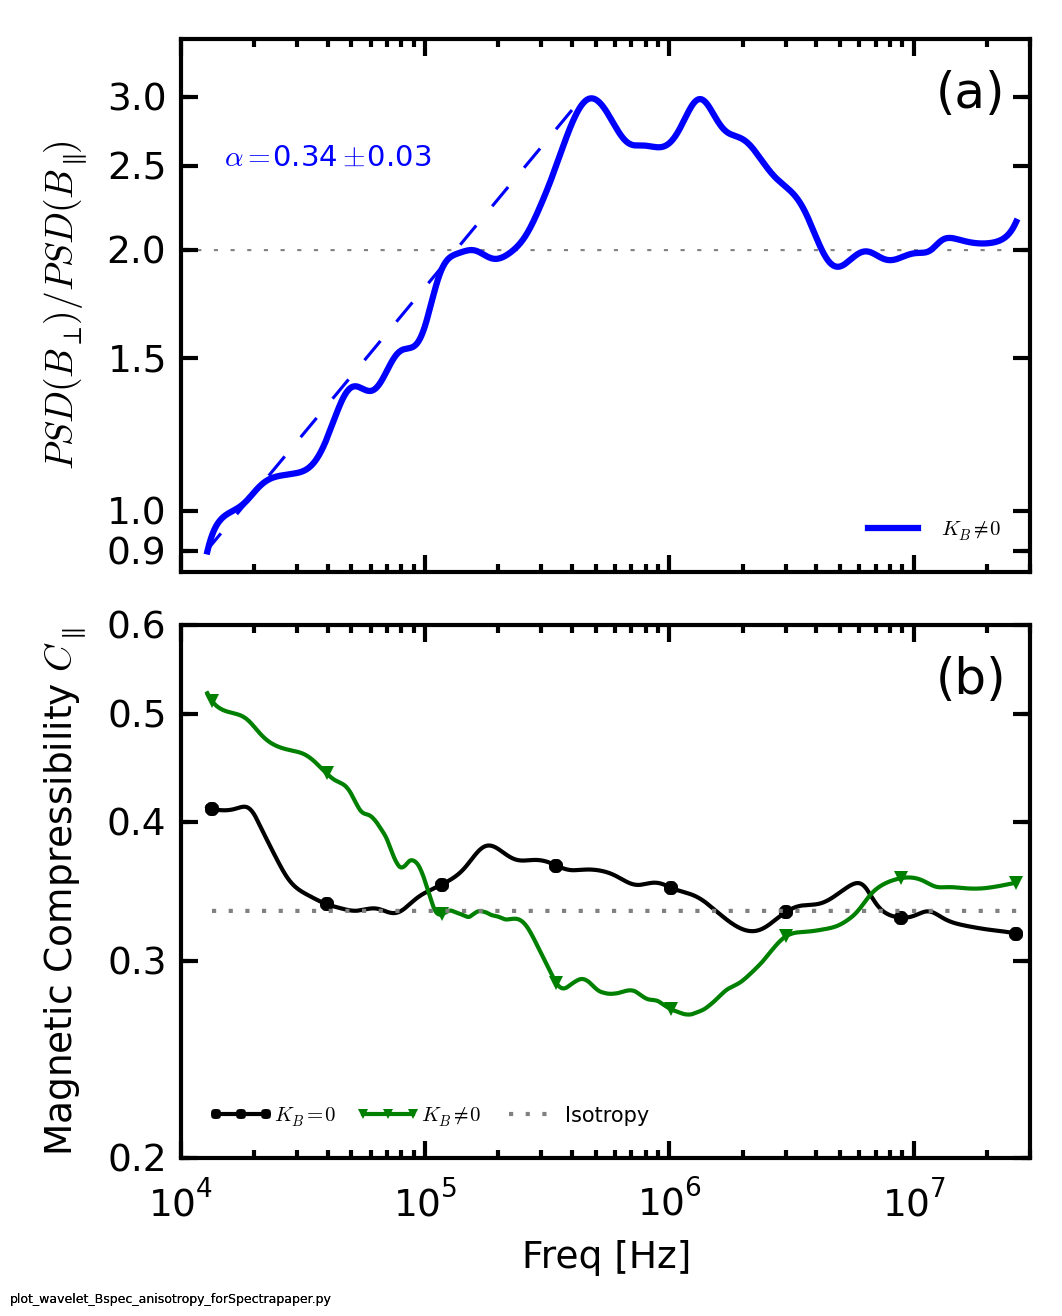
\includegraphics[width=8.5cm]{mag_compressibility_0helchan1t4prelim_1helchan1t6Kiydef_wratio_wfit}}
\caption{\label{fig:fitratio}}
\end{figure}

\begin{figure}[!htbp]
\centerline{
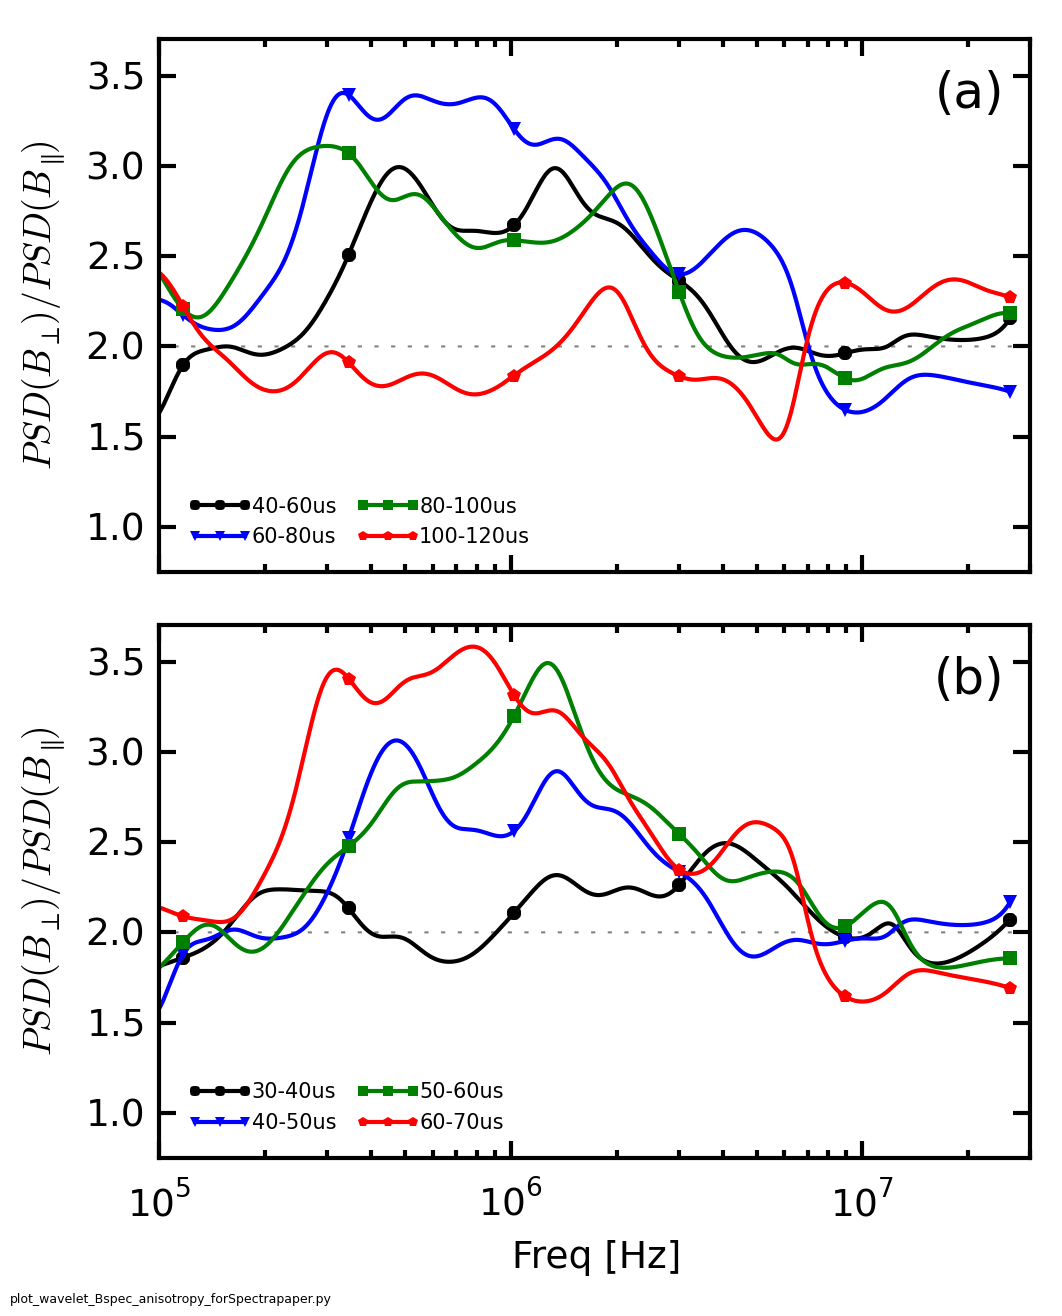
\includegraphics[width=8.5cm]{Bperppara_chan1t4_1mWbspectra_timescan}}
\caption{\label{fig:timeratio}}
\end{figure}

Fits to both the spectra and the ratio are shown in figure~\ref{fig:spectra}. In figure~\ref{fig:spectra}(a), fits are made to four sections of each curve. The spectral indices, error and range of fit for both parallel and perpendicular spectra are shown in the table below. Overall, the spectral indicies are anisotropy; for each section fit, the parallel slope is consistently steeper than the perpendicular slope. This difference is also reflected in the fit shown in figure~\ref{fig:fitratio}(a). An index of $\alpha = 0.35$ indicates that the ratio scales like $f^{1/3}$ for the region between 10kHz and 500kHz.

\begin{table}
\caption{\label{tab:Bindices}Indices from MLE power-law fits of magnetic fluctuation spectra in Figure~\ref{fig:spectra}.}
\begin{tabular}{cccc}
\toprule
Fit Range[MHz]	&	Direction		&	Index	&Error\\
\hline
0.01-0.1				& $\parallel$	& 1.27	&0.07\\
								& $\perp$			& 1.05  &0.07\\
\hline
0.07-0.3				& $\parallel$	& 2.66	&0.14\\
								& $\perp$			& 2.33  &0.13\\
\hline
0.3-1.0					& $\parallel$	& 3.22	&0.19\\
								& $\perp$			& 3.00  &0.18\\
\hline
1.5-10					& $\parallel$	& 4.91	&0.19\\
								& $\perp$			& 5.19  &0.20\\
\hline
\end{tabular}
\end{table}

An alternate presentation of this ratio is shown in figure~\ref{fig:fitratio}(b), where the ratio of perpendicular and parallel fluctuation power is cast in terms of magnetic compressibility~\cite{kiyani13},
\begin{equation}
C_{\parallel}(f) = \frac{1}{N}\sum^{N}_{j=1}\frac{B_{\parallel}(t_{j},f)}{B_{\parallel}(t_{j},f)+B_{\perp}(t_{j},f)}
\label{eq:magcompress}
\end{equation}
which relates the anisotropy to the characteristic stiffness of the magnetic field structure. Note the ratio between parallel and total is taken before the Wavelet spectra are summed over the time range with this definition while the pure ratio shown in previous figure is taken after integration over time. This metric can be used to help unravel the nature of the fluctuations~\cite{tenbarge12,kiyani13}.

An evolution of the anisotropy over time is also observed. Figure~\ref{fig:timeratio}(a) and (b) shows the change of the anisotropy ratio as a function of time ranges of 10$\mu s$ intervals(a) and 20$\mu s$ intervals(b). The black curve in figure~\ref{fig:timeratio} shows a period of time, 30-40$\mu s$, just as the plasma is reaching the midplane probe. The curve remains near isotropic levels for most of the frequencies. As time increases in 10$\mu s$ intervals, the perpendicular power clearly increases in the 100kHz to 1MHz range, while decreases in the 10-100kHz range. The actually peaks highest in the time frame just beyond the main analysis period shown in figure~\ref{fig:spectra}(b). These trends demonstrate that the anisotropy increases as more time is allowed for the turbulence to evolve. Figure~\ref{fig:timeratio}(b), shows that after energy is no longer being injected to maintain the turbulence, the anisotropy decreases. After 100$\mu s$, the magnetic field fluctuations have return to isotropy.

\section{Flow and Density Spectra}

For a turbulence cascade to develop, a system needs both energy injection and energy dissipation. The separation of spatial scale between injection and dissipation determines the size of the inertial range. While the actual injection mechanisms of the solar wind are not completely understood, there is evidence from the comparison of large scale magnetic field and velocity fluctuation data that velocity fluctuation energy is being tapped by magnetic fluctuations to sustain an injection-range like cascade for magnetic spectra~\cite{roberts10}. In the SSX plasma, however, the injection scale energy is primarily magnetic---the formation of the unstable spheromaks. This is borne out by similar comparisons of magnetic spectra and velocity spectra. Figure~\ref{fig:BvsFlow} shows magnetic spectra (a) and Mach number fluctuation spectra (b) for two plasma states: a high and low magnetization state.

\begin{figure}[!htbp]
\centerline{
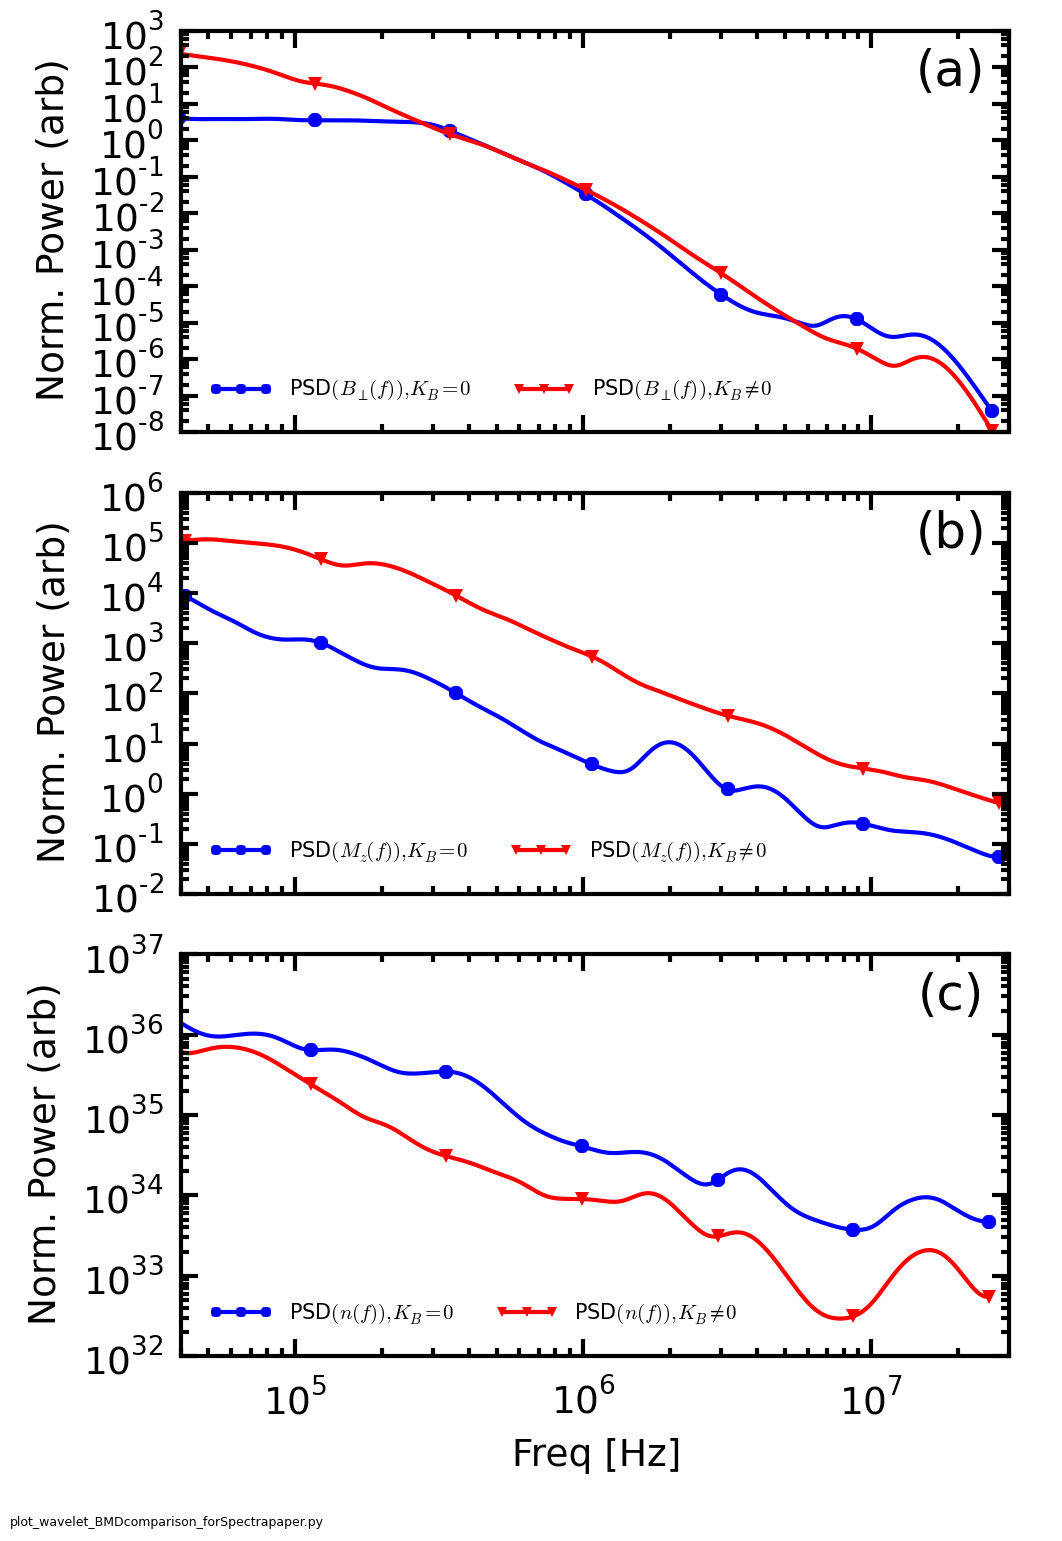
\includegraphics[width=8.5cm]{BvsFlowvsDensspec_2fluxes_separateplots_40t60us}}
\caption{\label{fig:BvsFlow}}
\end{figure}

Comparison of the blue and purple curves in Figure~\ref{fig:BvsFlow}(a) show the affect on large scale fluctuations from the presence of a strong initial magnetic field. Comparing these states with the respective velocity fluctuations shows how the additional magnetic energy injection at larger scales affects the velocity. For the low field state, the velocity cascade is immediately steep as well as lower in energy overall. In the high field state, however, the velocity fluctuation scaling is shallower, but then has a breakpoint around the frequency where B-field fluctuation energy is about the same between high and low field states. This suggests that the state with more injected magnetic energy delivers some of its energy to the velocity fluctuations.

\begin{figure}[!htbp]
\centerline{
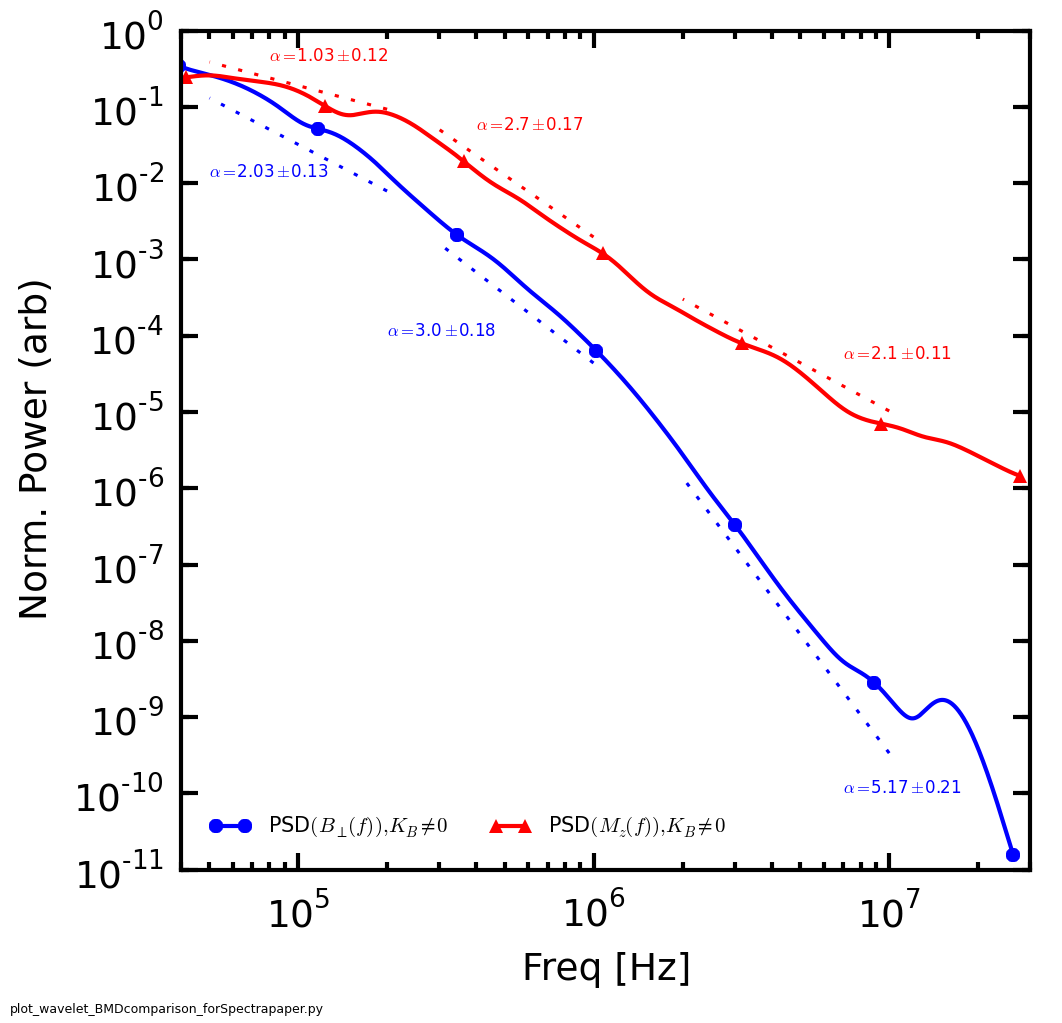
\includegraphics[width=8.5cm]{BvsFlowspec_wFits_40t60us}}
\caption{\label{fig:BvsFlow_wFits}}
\end{figure}

This can be seen quantitatively in Figure~\ref{fig:BvsFlow_wFits} which puts the high field magnetic and velocity fluctuation spectra on the same relative scale. The velocity spectra scales like $f^{-1}$ about to about 200kHz, a scaling which is typical for injection range turbulence. Meanwhile, the magnetic spectra is steeper, which implies that some of the magnetic energy may be going to drive flows, though the exact mechanism of this energy transfer is not known and its study is reserved for later work.

\begin{table}
\caption{\label{tab:Bindices}Indices from MLE power-law fits of magnetic and Mach number fluctuation spectra in Figure~\ref{fig:BvsFlow_wFits}.}
\begin{tabular}{cccc}
\toprule
Fit Range[MHz]	&	Parameter		&	Index	&Error\\
\hline
0.05-0.2				& $M_{z}$			& 1.03	&0.12\\
								& $B_{\perp}$	& 2.03  &0.13\\
\hline
0.3-1.0					& $M_{z}$			& 2.70	&0.17\\
								& $B_{\perp}$	& 3.00  &0.18\\
\hline
2.0-10					& $M_{z}$			& 2.10	&0.11\\
								& $B_{\perp}$	& 5.17  &0.21\\
\hline
\end{tabular}
\end{table}

Beyond 200kHz, the velocity fluctuations scaling steepens suggesting an inertial range scale. The B-field steepens further as well. Beyond, 2MHz, the B-field scaling drops off significantly while the velocity spectra scaling actually slightly increases. This is possibly due to a dissipation mechanism that may be further tapping magnetic energy, and given the increase in velocity spectra scaling, even further adding to velocity fluctuation energy. It may, however, also be due to the frequency of response of the Mach probe itself. Alternative velocity fluctuation measurements are being considered (i.e. electric field fluctuations) for future runs for comparison.

\section{Wavenumber Spectra}

A unique turbulence measurement that can be made in the SSX plasma is a direct wavenumber spectrum using a multi-tipped magnetic probe that is inserted radially into the wind-tunnel. The probe can measure $\vec{B}(t)$ at 16 locations along a 6.8cm length of the radius at a spacing of 0.4572cm. In Fourier space, this allows measurements of scales from about 7cm to 1cm. Given that the injection scale of the magnetic energy is on the order of the initial size of the spheromaks---15.5cm---and a dissipation scale can be estimated to be just under 1cm---ion inertial length for a 1.5$\times 10^{15}$cm$^{-3}$ plasma is on the order of 0.6cm---the spatial range sampled by the probe can be assumed to be in the inertial range.

Since the probe can take simultaneous measurements of $\vec{B}$ across the plasma, snapshots of the spatial structure of the plasma can be made at each time step. In turn, these spatial distributions can be Fourier transformed to produced power-spectra of the scales. Thus, this measurement can capture the direct wavenumber spectra of the plasma turbulence without reliance on any Doppler shifting as is needed to invoke the Taylor Hypothesis. Moreover, since $\vec{B}$ is constructed from three orthogonal measurements, the power-spectra of vectors perpendicular and parallel to the axial flow of the plasma can be separately analyzed. 

The downside, of course, to a measurement of the wavenumber spectra in this way is the lack of resolution compared to a Doppler-shifted frequency spectrum. With only 16 spatial points, the Fourier spectrum can have only 8 points, and only seven can be displayed in log-log format. However, despite this lack of resolution, it is a more physical direct measurement and can the measurement can still be used to cross-reference other observations of spectra.

\begin{figure}[!htbp]
\centerline{
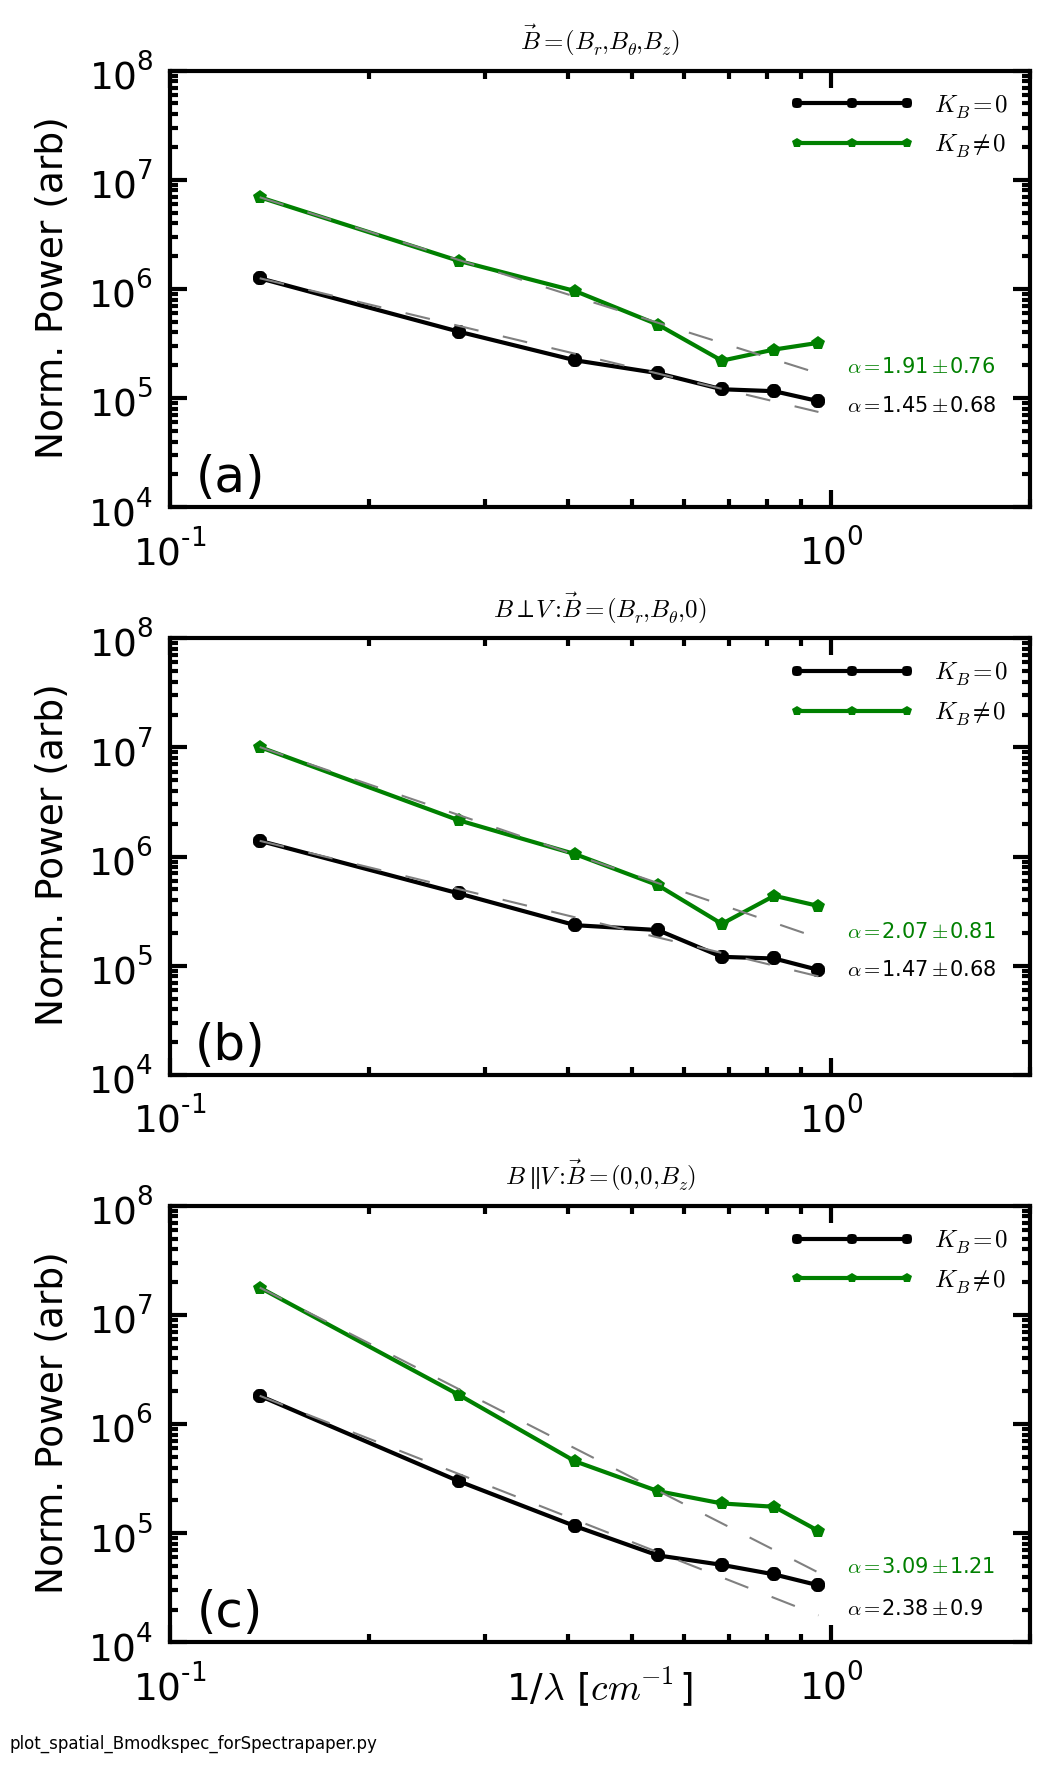
\includegraphics[width=8.5cm]{Bmod_FFTwavenumberspectra_wFits_40t60us}}
\caption{\label{fig:wavenumber_spectra}}
\end{figure}

Figure~\ref{fig:wavenumber_spectra} shows the wavenumber power spectrum for three different helicity states and for full-vector(a), perpendicular vector(b) and parallel vector(c), averaged for each timestep in between 40 and 60$\mu s$ and over 40 shots. Comparison of the three curves in Figure~\ref{fig:wavenumber_spectra}(a) seem to show a slight variation in slope as the helicity state is increased, though with the large given errors in the fit (due to low resolution), the slopes of all three curves are essentially the same. A similar trend is observed amongst the three curves in (b) and (c) as well. A larger difference arises when comparing the curves of different vectors. Namely, the separately computed perpendicular and parallel spectra in (b) and (c) tend to be slightly steeper than the full vector spectra in (a). Moreover, the parallel curves appear to be steeper than the perpendicular curves. Again, the error in the fits are large for the low resolution data, but the trends are very suggestive.

\begin{figure}[!htbp]
\centerline{
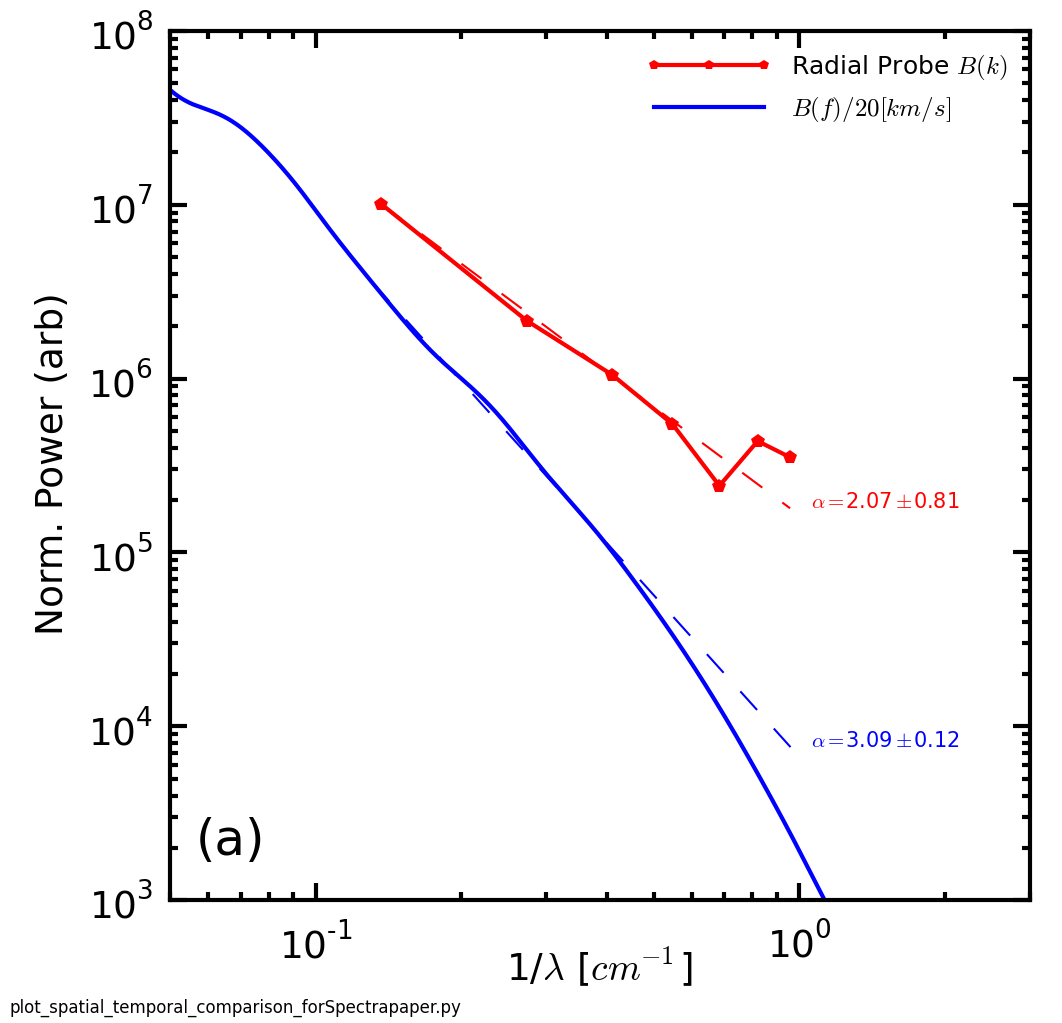
\includegraphics[width=8.5cm]{B_spatial_temporal_comp_wFits_40t60us}}
\caption{\label{fig:wavenumber_comp}}
\end{figure}

The wavenumber spectra and frequency spectra can be directly compared by invoking the Taylor hypothesis for the frequency spectra and Doppler-shifting the frequency spectra by the bulk plasma velocity,
\begin{equation}
B(f) \longrightarrow B(f-kV_{p}) \longrightarrow V_{p}B(k)
\label{eq:Taylor_Hyp}
\end{equation}

For this plasma, the velocity can be estimated (using both time-of-flight and Mach probe measurements) to be about 20km/s. If the frequency portion is ignored in Equation~\ref{eq:Taylor_Hyp}, the frequency spectra can be plotted on the same scale as the wavenumber spectra. Figure~\ref{fig:wavenumber_comp} shows this comparison for the 1mWb stuffing flux plasma. The curves are placed arbitrarily on the y-axis. Maximum likelihood estimation power-law fits are made to the same range in both curves. The slopes of the curves are comparable suggesting that invoking the Taylor hypothesis for the frequency spectra is not entirely unwarrented. Instead, the steeper slope of the frequency spectra could be reflective of the effect of a combined temporal {\it and} spatial scaling, which the direct wavenumber spectrum does not include. However, breakdown of Taylor Hypothesis has been shown to make the spectra more shallow than steeper(Klein Taylor Hypotheis draft). The differences might also be reflective of a wavenumber anisotropy as the direct wavenumber spectra probes $k_{r}$ and the Doppler-shifted frequency spectra probes $k_{z}$.

\section{Comparison with Simulation}

Simulations of the plasma produced in the SSX wind-tunnel have been generated with the HiFi spectral-element multi-fluid modeling framework using a set of normalized compressible Hall-MHD equations. Favorable comparisons of turbulent spectra and intermittency have been reported between these simulations and the experimental plasma~\cite{schaffner14a}. Further analysis is presented here which show similar observations of anisotropy, wavenumber spectra, and velocity-B-field spectra comparisons as is seen in the experiment.

Timeseries of quantities in 3mm spheres approximately 1cm off the central axis and at the midplane are extracted from the simulation for density, three axes of magnetic field, three axes of velocity. To provide some ensemble averaging, points at eight different azimuthal angles are used.

\begin{figure}[!htbp]
\centerline{
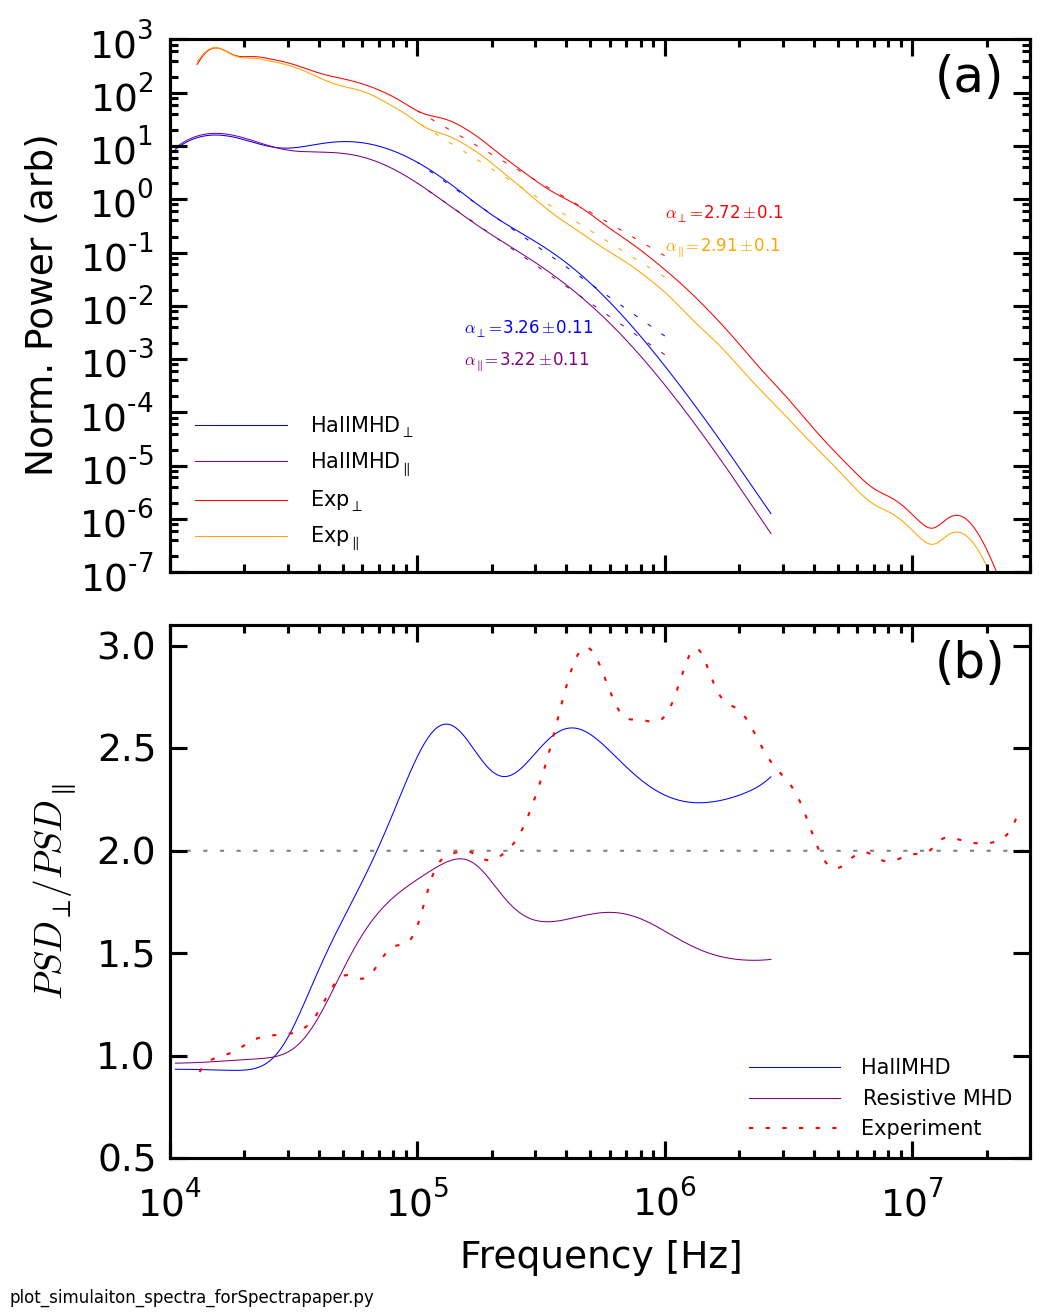
\includegraphics[width=8.5cm]{Anisotropy_simulation_comparison}}
\caption{\label{fig:aniso_comp}}
\end{figure}

\begin{table}
\caption{\label{tab:Bindices}Indices from MLE power-law fits of magnetic fluctuation spectra from experiment and simulation in Figure~\ref{fig:aniso_comp}.}
\begin{tabular}{cccc}
\toprule
Fit Range[MHz]	&	Parameter						&	Index	&Error\\
\hline
0.1-1.0					& Sim:$B_{\parallel}$	& 3.22	&0.11\\
								& Sim:$B_{\perp}$			& 3.26  &0.11\\
								& Exp:$B_{\parallel}$	& 2.91	&0.10\\
								& Exp:$B_{\perp}$			& 2.72  &0.10\\
\hline
\end{tabular}
\end{table}

The simulation timeseries data is analyzed in a similar was the the experimental data with the exception that the mother wavelet used for the wavelet transform of the simulation data is a fourth-order Paul rather than a sixth-order Morlet, in order to better capture time resolution for the lesser sampled simulation. A variance anisotropy analysis is conducted in the same manner as well using a local magnetic field and the projection method. Figure~\ref{fig:aniso_comp}(a) shows simulation decomposition into perpendicular and parallel spectra compared to experimental spectra using the 1.0mWb stuffing data. The simulation and experimental spectra are staggered placed on the y-axis to emphasize features of the shape. Clearly, the simulation data exhibits growing variance anisotropy with increasing frequency. The slopes of the simulation spectra match qualitatively well in the region of 100kHz to 1MHz, though the fit spectra indices indicate a slightly steeper slope than the experiment. The high frequency end of the simulation spectra drops in power faster than the experiment, likely due to the limits in time resolution.

The trend in anisotropy ratio is also similar in the simulation and the experiment, as seen in Figure~\ref{fig:aniso_comp}(b), though the simulation does not reach as large a peak ratio, nor does it scale at quite the same rate. Nevertheless, the clear observation of increase an increase in ratio suggests that the compressible Hall-MHD physics captures the generation of the anisotropy. Figure~\ref{fig:aniso_comp}(b) also shows the anisotropy ratio for a simulation run with the Hall term in the compressible MHD equations set to zero. Unlike the Hall MHD and the experiment, the ratio does not switch over to perpendicular dominance, and instead stays near or below the isotropy line. The implications of this have not been analyzed in depth.

\begin{figure}[!htbp]
\centerline{
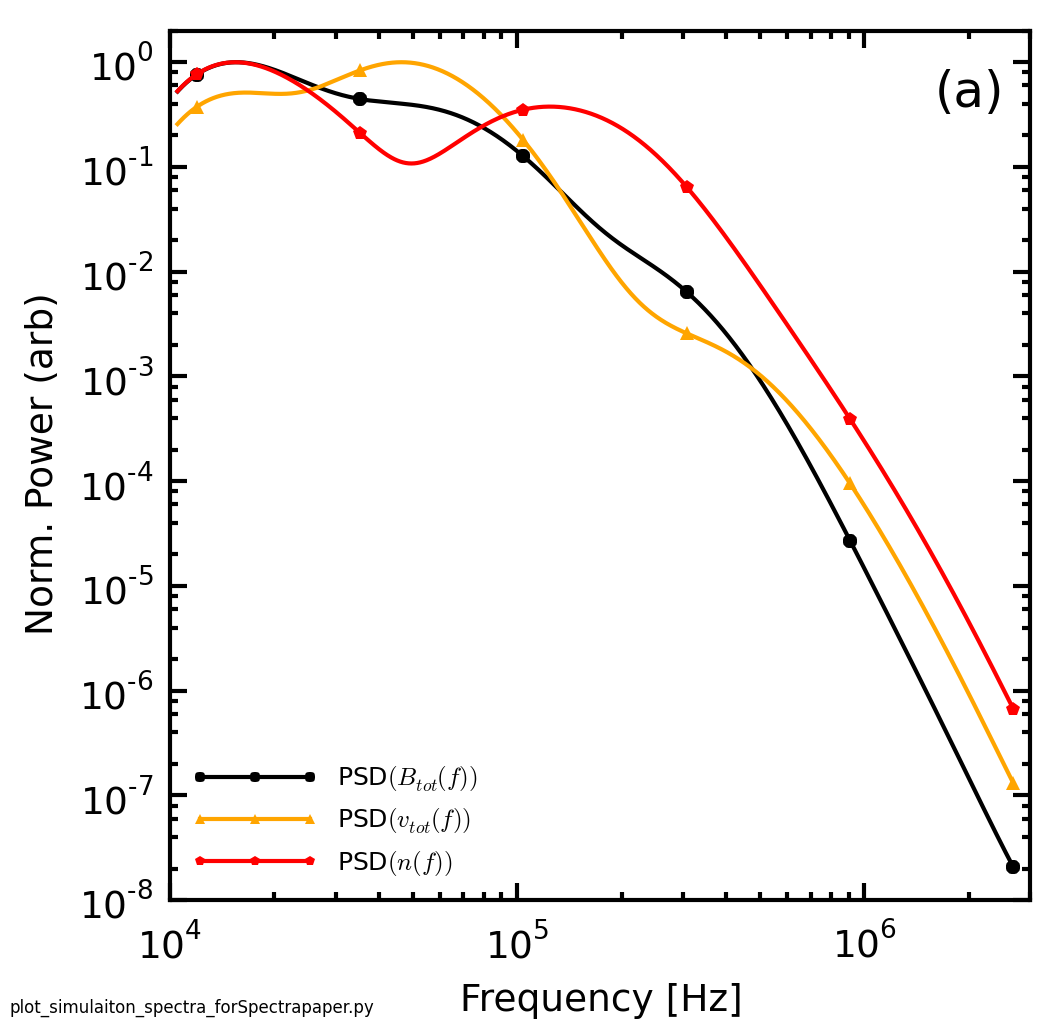
\includegraphics[width=8.5cm]{BfieldFlow_simulation_comparison}}
\caption{\label{fig:bflow_comp}}
\end{figure}

A comparison between velocity and magnetic field fluctuations in the simulation can also be made. Figure~\ref{fig:bflow_comp} shows wavelet transformed frequency power spectra for the total magnetic field (sum of $B_{r}$, $B_{\theta}$, and $B_{z}$), total velocity, and density, all normalized to their respective peaks. Qualitatively, the comparison between velocity and magnetic field spectra supports the results of the experimental data for stuffed plasmas: the peak in the velocity spectra occurs at a larger frequency than the magnetic spectra. This suggests that energy for the velocity fluctuations are being injected at a smaller scale than the magnetic field fluctuations. Though not conducted here, further analysis of the simulation could potentially show direct energy transfer between the magnetic and velocity fluctuations.

\begin{figure}[!htbp]
\centerline{
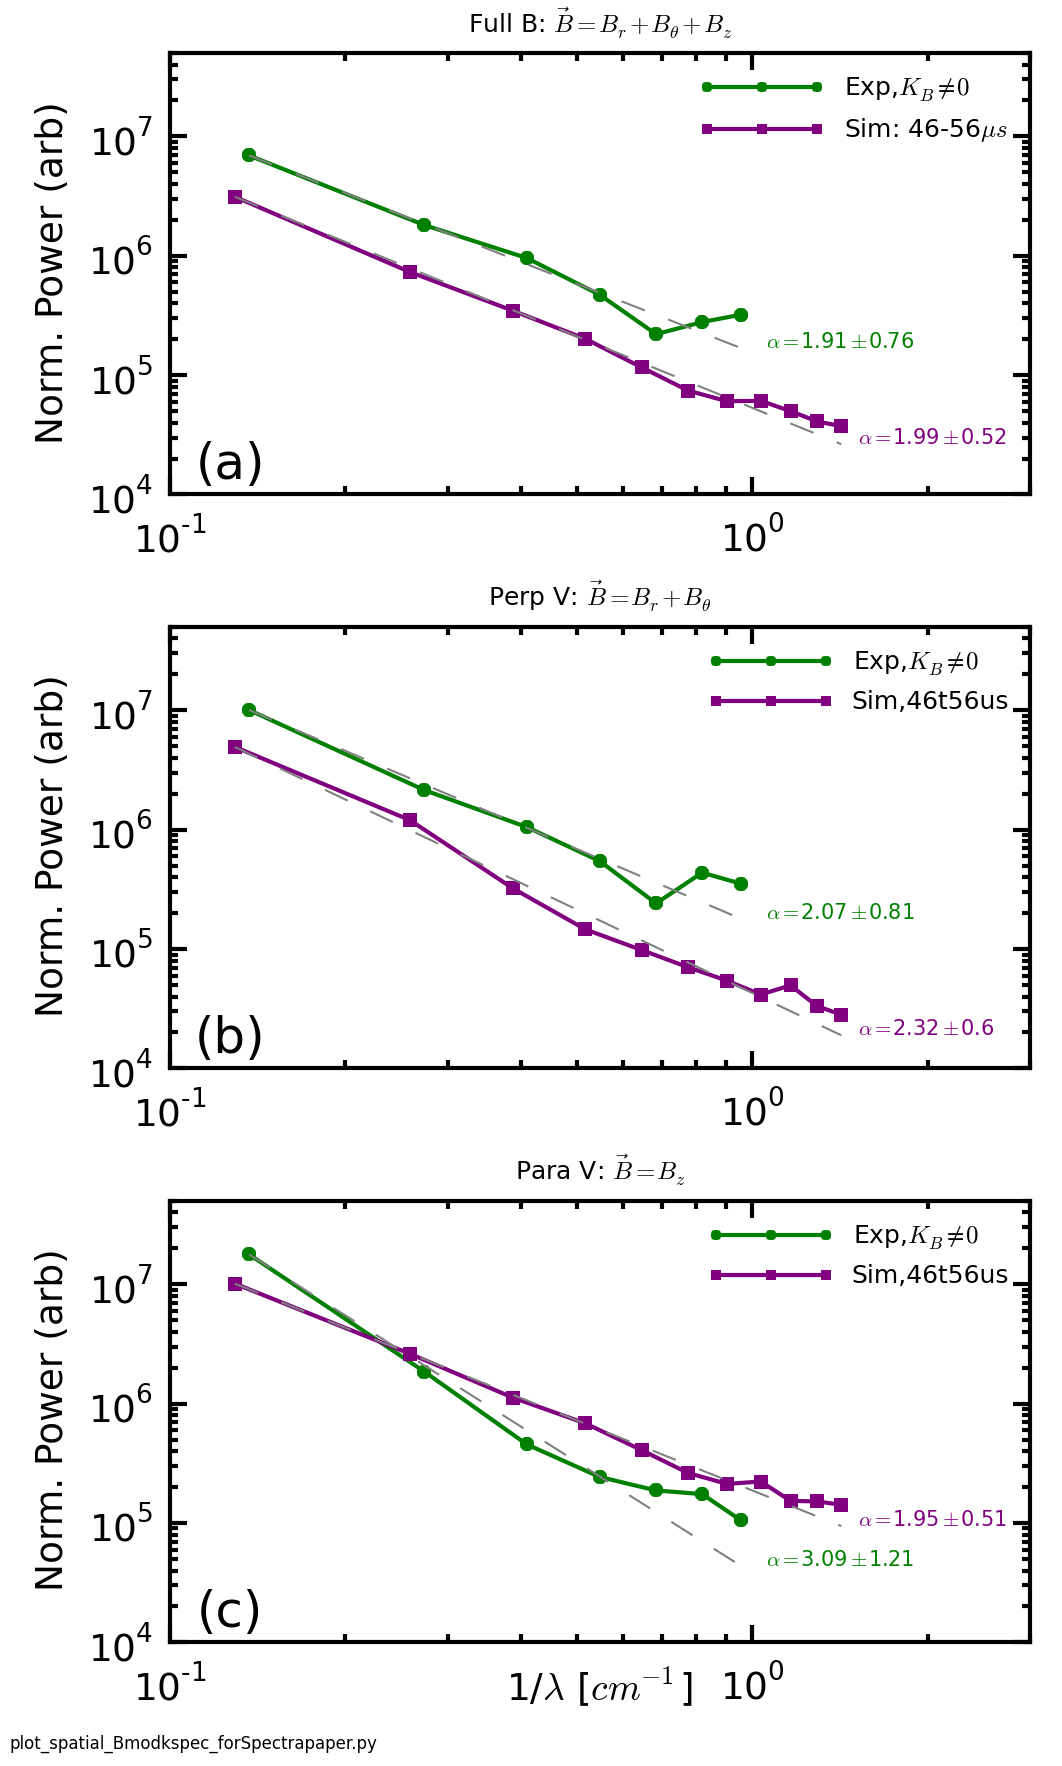
\includegraphics[width=8.5cm]{Bmod_FFTwavenumberspectra_wFits_40t60us_simulationcomparison}}
\caption{\label{fig:sim_wavenumber_comp}}
\end{figure}

\begin{figure}[!htbp]
\centerline{
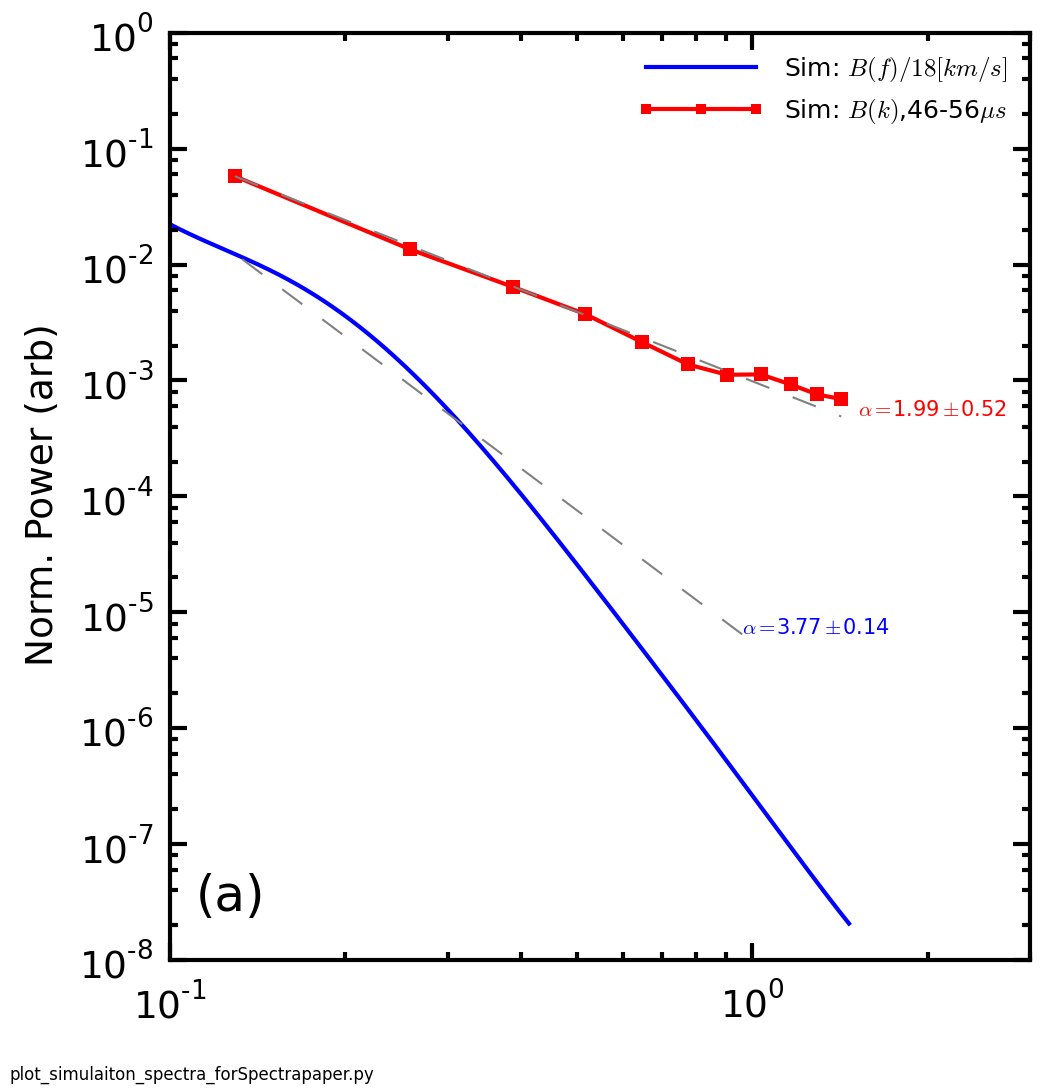
\includegraphics[width=8.5cm]{Simulation_spatial_temporal_spectra_comparision}}
\caption{\label{fig:sim_spatial_comp}}
\end{figure}

The wavenumber spectra from a radial cut of the simulation data is also generated using 24 points. Figure~\ref{fig:sim_wavenumber_comp} shows a direct comparison between simulation and experimental wavenumber spectra. The slightly smaller separation between distances allows the simulation to reach a smaller scale than the experiment, to about 0.7cm. In general, the comparison between simulation and experiment is good suggesting that the simulation is capturing well the spatial structure of the turbulence. Even though the simulation can observe slightly smaller scales, it does not appear to probe small enough to exhibit any dissipation effects at to ion inertial length scales which for the simulation is at about 0.7cm.

Like in the experiment, the spatial and temporal spectra of the simulation is compared and shown in Figure~\ref{fig:sim_spatial_comp}. The simulation has a bulk axial flow of 18km/s, close to the 20km/s observed in the experiment. A similar trend is seen with the spatial spectra having a shallower slope than the Doppler-shifted frequency spectra. The main difference again appears to be that the frequency spectra hits the limits of the temporal resolution at larger frequencies than the experiment.

These further comparisons of turbulent statistics and characteristics between the experimental plasma and a compressible Hall-MHD simulation help validate the model as useful for understanding the physical processes. Subsequent simulation analysis will likely entail more detailed computation of how energy might be being distributed and moved through the plasma including relationships between magnetic field and velocity as well as between magnetic fluctuations perpendicular and parallel to a local B-field.

\section{Discussion and Evidence for Ion Scale Effects}

\begin{figure}[!htbp]
\centerline{
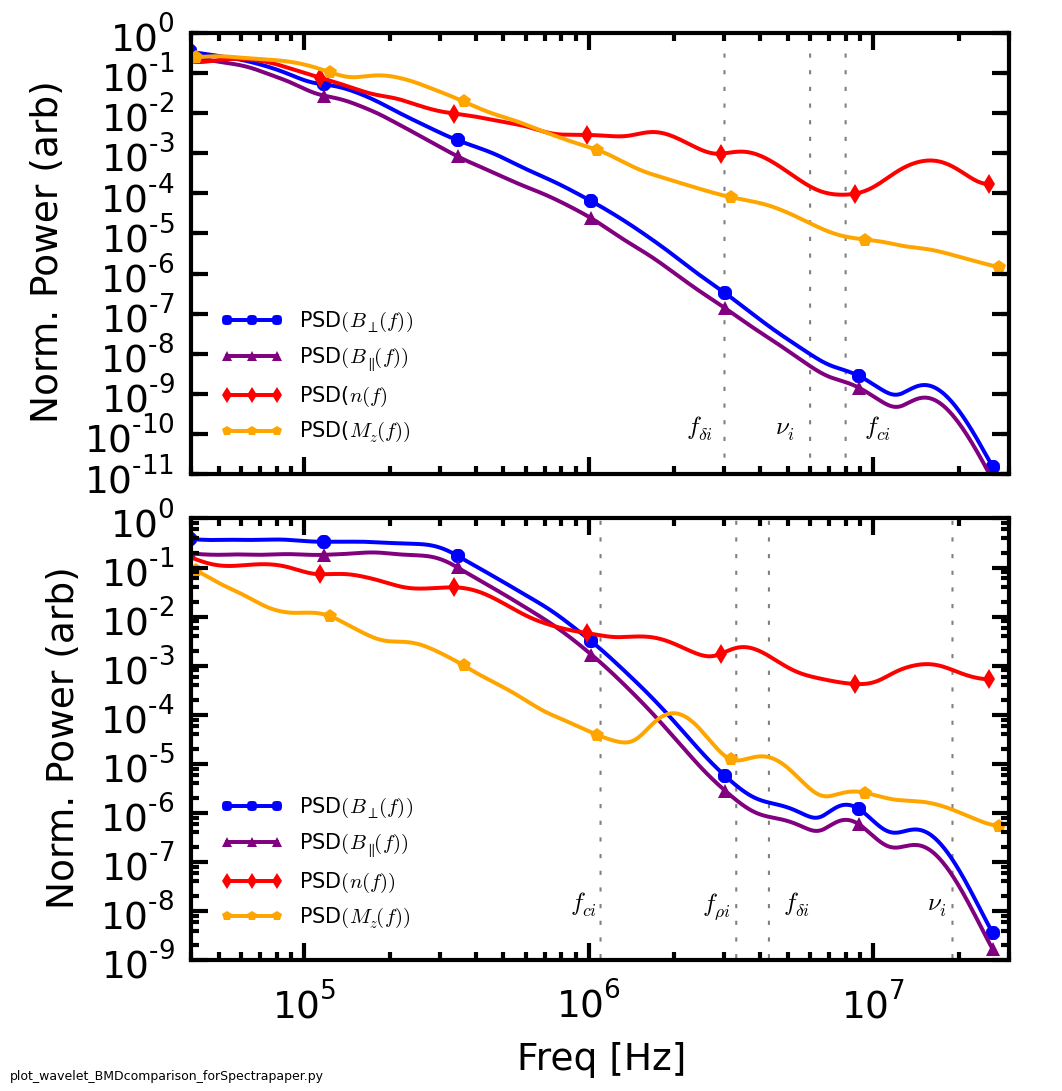
\includegraphics[width=8.5cm]{BvsDensvsFlowspec_1mWb_and_0mWbcomp_40t60us}}
\caption{\label{fig:BMD_comp}}
\end{figure}

%1mWB run
%dens 1.39e15 cm^-3
%bfield 5283 G
%Ti = 23 eV
%bulk flow = 20km/s

%results
%Va = 309km/s
%Beta = 0.07
%Cs = 31km/s
%f_i = 8MHz
%nu_i = 6MHz
%rho_i = 0.09cm
%c/w_pi = 0.61cm
%ion_mfp = 0.16cm
%doppler shifted c/wpi = 3MHz
%doppler shifted rho_i = 20MHz

%0mWb run
%dens 2.84e15 cm^-3
%bfield 747 G
%Ti = 17 eV
%bulk flow = 20km/s

%results
%Va = 30km/s
%Beta = 5.5
%Cs = 31km/s
%f_i = 1.1MHz
%nu_i = 19MHz
%rho_i = 0.56cm
%c/w_pi = 0.43cm
%ion_mfp = 0.05cm
%doppler shifted c/wpi = 4.3MHz
%doppler shifted rho_i = 3.3MHz

\begin{table}
\caption{\label{tab:params}MHD wind tunnel plasma parameters during the equilibrium epoch for the present configuration of SSX.}
\begin{tabular}{|l|l|l|}
\hline
Parameter&1.0mWb&0.0mWb\\
\hline
$Measured$&&\\
\hline
$\langle |B|\rangle [kG]$&5.283&0.747\\
$\langle n\rangle \times 10^{15} [cm^{-3}]$&1.39&2.84\\
$\langle T_{i}\rangle [eV]$&23&17\\
Bulk Flow $[km/s]$&20&20\\
\hline
$Computed$&&\\
\hline
$\beta$&0.07&5.5\\
$V_{a} [km/s]$&309&30\\
$C_{s} [km/s]$&31&31\\
$\rho_{i} [cm]$&0.09&0.56\\
$\delta_{i} [cm]$&0.61&0.43\\
$\lambda_mfp^{i} [cm]$&0.16&0.05\\
$f_{ci} [MHz]$&8&1.1\\
$\nu_{i} [MHz]$&6&19\\
$f_{\delta i} [MHz]$&3&4.3\\
$f_{\rho i} [MHz]$&20&3.3\\
\hline
\end{tabular}
\end{table}

A major remaining question for this analysis is whether the plasma diagnostics are able to observe effects of a dissipation scale in this turbulence. Perhaps, a more general question can be posed in how well does this plasma exhibit a traditional fluid-turbulence-like picture which posits an injection scale, inertial scale and dissipation scale.

The results of this analysis provide a number of hints that the ion inertial scale length is being probed, but no one piece of evidence is strong enough to make a conclusive assertion. The first clue arises by comparing the break-point of the magnetic spectra with the Doppler-shifted ion inertial scale length, $f_{\delta i}$. Figure~\ref{fig:BMD_comp}(a) shows the spectra for magnetic field, Mach number and density for the 1.0mWb run all normalized to their respective maximum value, with dashed lines indicating the Doppler-shifted frequency of ion inertial length, $f_{\delta i}$ using a bulk flow speed of 20km/s, the collision frequency, $\nu_{i}$, and ion cyclotron frequency, $f_{ci}$. Note that the break point occurs just before the ion inertial frequency is reached. Since the ion inertial scale is often associated with the scale size of reconnection layers or current sheets, a break-point just proceeding this scale suggests the onset of a dissipation mechanism associated with current sheets of some form(citation needed).

Two supporting pieces of evidence for this hypothesis come from the comparison of the density and magnetic spectra as well as the trend in variance anisotropy. The red curve in Figure~\ref{fig:BMD_comp}(a) shows a slight bump up again around $f_{\delta i}$. This is possibly evidence of the density bump effect observed when the plasma becomes more compressible---which would be expected at ion inertial length scales. Similarly, the anisotropy ratio becomes to decrease at about this frequency (see Figure~\ref{fig:fitratio}) which also suggests an increase in compressibility (or really, decrease of incompressibility.)

However, there remain other explanations for these effects. One, the Taylor Hypothesis used to establish the connection between the frequency and the scale length here is not obviously valid. If the Taylor Hypothesis cannot be invoked, there may be other reasons for the break-point observed. Also, the density bump seen in Figure~\ref{fig:BMD_comp}(a) may be due to noise contamination at these scales rather than a real effect.

Comparison of the two different helicity states only adds to the ambiguity. Figure~\ref{fig:BMD_comp}(b) shows the same curves as in (a), but for the unstuffed/zero-helicity state. The break-point in the magnetic field here appears to occur close to the ion cyclotron frequency rather than the ion inertial length. It should be noted though that previous work~\cite{schaffner14b} has suggested that the zero-helicity state consists of much fewer current sheets and as such, dissipation in this state would depend much less on those mechanisms. The zero-helicity state also shows no change in anisotropy with scale nor any density bump.

The results presented, nevertheless, do highlight the need for further investigation, particularly in whether a Taylor Hypothesis can be invoked, or the very least, whether some time of Doppler shift can be applied to properly connect the frequency and scale size of the signal. Similarly, a higher resolution in the spatial probes could provide confirmation as its current state just misses the apparent dissipation scale. Moreover, better resolved density and Mach flow diagnostics would be useful in order to distinguish between noise and real effect.

Lastly, the simulation angle can potentially provide some explanation of the physics occurring. Unfortunately, the simulation appear to not probe at a small enough scale to show ion scale effects. Both the frequency spectra and wavenumber spectra fall short ion inertial scales. The variance anisotropy ratio supports this as an increase in the ratio is observed, but not a decrease at smaller scales/higher frequencies. However, the favorable comparison between the experiment and the simulation at smaller frequencies and larger scales means that improvement of the simulations resolution maybe be useful for exploring the dissipation physics.

\section{Conclusions}



\appendix

\section{Computation of Variance Anisotropy}

The computation of the variance anisotropy involves two main steps: a determination of fluctuation power and an estimate of the distribution of the fluctuation power relative to a vector direction. The first step is accomplished using a Wavelet transform procedure as is discussed in the text. The division of fluctuation power is accomplished using what will be described here as a projection method. A second estimate of fluctuation power distribution is constructed using a threshold method and is also described in detail in this appendix. The threshold method is a more straightforward process for determining the level of variance anisotropy, but suffers from diminishing resolution. Its presentation here is mainly as a validation of the eventual use of the projection method for the analysis in the paper. 

\subsection{Threshold Method}

Both the threshold method and the projection method for determining variance anisotropy rely on the ability of the wavelet transform to yield a power spectrum distribution (PSD) as a function of both time and frequency (i.e. B(f,t)). A local (in time) vector $\vec{B}$ is determined for each time, t,
\begin{equation}
\vec{B}(t) = B_{r}(t)\hat{r} + B_{\theta}(t)\hat{\theta} + B_{z}(t)\hat{z}
\label{eq:Bvector}
\end{equation}
where each component $n=r,\theta,z$ is determined from $\dot{B}_{n}$ by integrating over time as
\begin{equation}
B_{n}(t) = \int_{0}^{t} \frac{d}{d\tau}B_{n}(\tau)d\tau.
\label{eq:Bintegrated}
\end{equation}

Since the magnetic probe measures orthogonal magnetic field directions by construction, this fact can be used to directly seek a difference in fluctuation spectra depending on orientation perpendicular or parallel to the overall field. Thus, a threshold magnitude for each component can be defined as a fraction of the total magnitude as in,
\begin{equation}
B_{n}^{threshold} \geq \frac{|B_{n}|^{2}}{|\vec{B}|^{2}}
\label{eq:Bthreshold}
\end{equation}
which reflects the relative amount that the total vector points in one of the three orthogonal directions. Then for every time, t, in a given time range and for each shot, the quantity $B_{n}(f,t)$ is summed for each t where
\begin{equation}
\frac{|B_{n}|^{2}}{|\vec{B}|^{2}} \geq B_{n}^{threshold}
\label{eq:Bcondition}
\end{equation}
for all frequencies, $f$. The value chosen for $B_{n}^{threshold}$ determines how strictly total vector aligns with the component, $n$. By definition, then, the summed power for $B_{n}$ is considered the parallel component and the sum of the remaining two directions is the perpendicular component. If there is any anisotropy in the signal, a difference in energy content of the spectra should become apparent as the threshold value is increased.

\begin{figure}[!htbp]
\centerline{
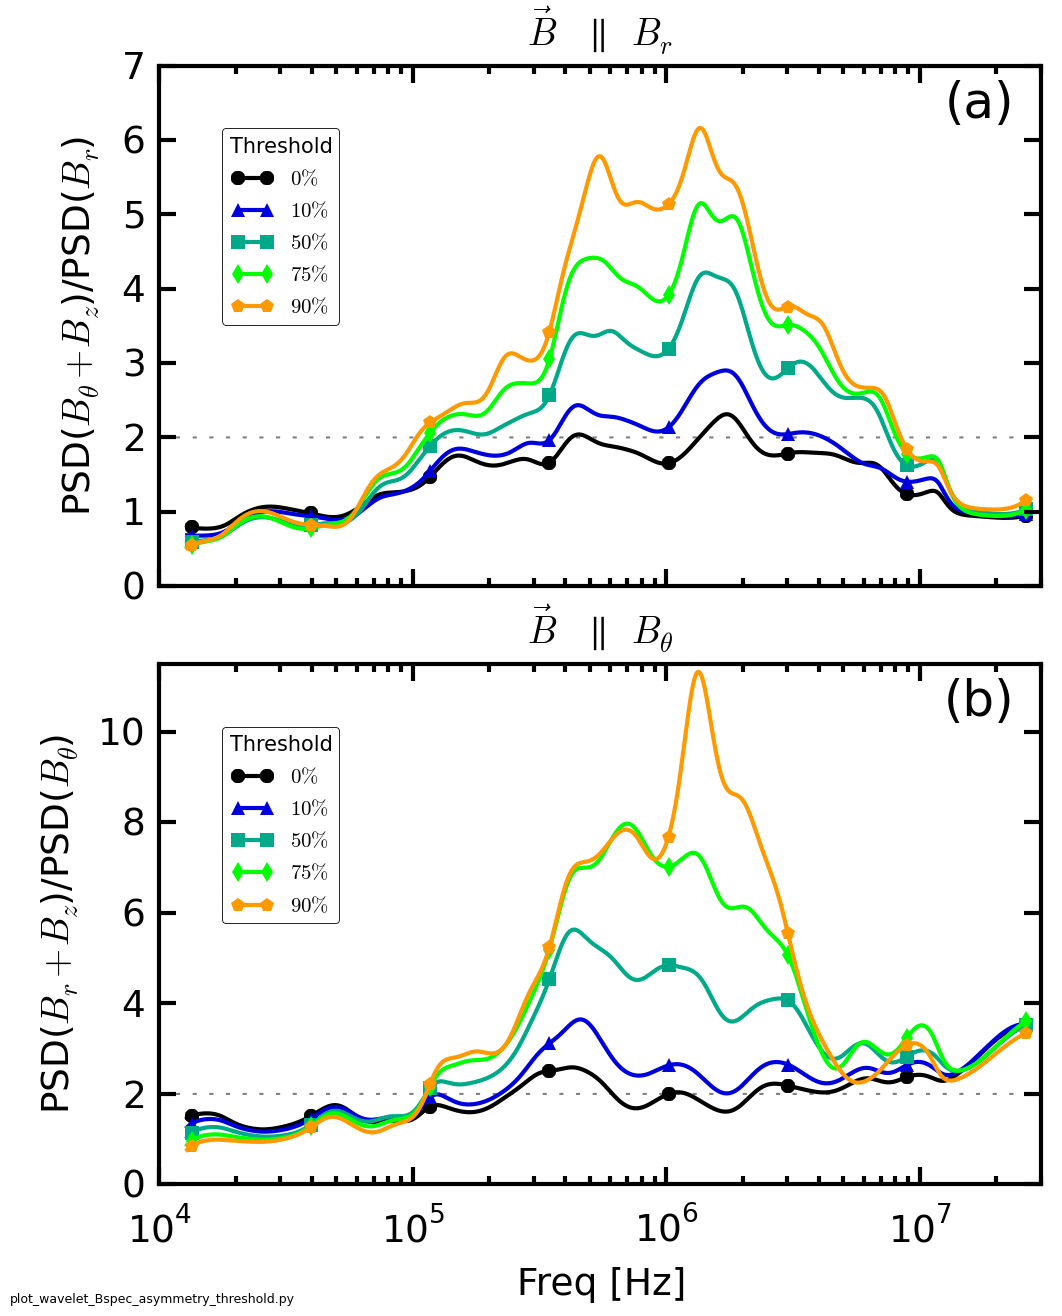
\includegraphics[width=8.5cm]{Bperppara_spectra_thresholdscan40t60us}}
\caption{\label{fig:thresholdmethod}}
\end{figure}

Indeed, an effect like this is observed. Figure~\ref{fig:thresholdmethod} shows the ratio of total perpendicular fluctuation power to parallel fluctuation power for $n = r$(a) and $n = \theta$(b). The threshold fraction is indicated by color. The dashed line at 2 represents isotropy---where the sum of 2 perpendicular components is about twice the power of the single parallel component. Clearly, for the lowest threshold value, the ratio remains close to the isotropy line for all frequencies as would be expected. As the threshold value is raised, the ratio from about 10kHz and higher begins to grow. This shows there is variance anisotropy in the plasma. If the plasma were isotropic, a difference between perpendicular and parallel spectra would not be seen. The anisotropy ratio reaches a maximum as the threshold nears 100\%. The drawback to this method, however, is that as the threshold is increased, the number of individual spectra summed is reduced which increases the error of each curve.

\subsection{Projection Method}

An alternative method, and that used to compute the results presented in this manuscript, uses the $\vec{B}$ timeseries data to project spectral power into perpendicular and parallel portions at each timestep. This projection method uses all the available timesteps and shots rather than making a cut like the threshold method. It will be shown later that the two methods give quantitatively similar answers for the amount of variance anisotropy.

The projection method also uses the Wavelet transform to compute B(f,t). However, that than use the $\vec{B}(t)$ as a threshold value, it is used as a reference vector to determine what fraction of the fluctuation power of $B_{r}(f,t)$, $B_{\theta}(f,t)$, and $B_{z}(f,t)$ is perpendicular or parallel to that vector. The parallel component of each $B_{x}(f,t)$ is found by computing the projection,
\begin{equation}
Proj_{u}v = \frac{\vec{v} \cdot \vec{u}}{||\vec{u}||}\vec{u}
\label{eq:projection}
\end{equation}
which shows that the magnitude of the component of $B_{x}$ parallel to $\vec{B}$ is
\begin{equation}
B_{x}^{\parallel} = \frac{B^{2}_{x}}{|\vec{B}|^{2}}.
\label{eq:para_mag}
\end{equation}
Then, the magnitude of the component perpendicular is
\begin{equation}
B_{x}^{\perp} = 1 - \frac{B^{2}_{x}}{|\vec{B}|^{2}}.
\label{eq:perp_mag}
\end{equation}
Using these projection coefficients, each Wavelet transform spectra, $B_{x}(f,t)$ for $x = r,\theta,z$, can be divided into $B_{x}^{\parallel}(f,t)$ and $B_{x}^{\perp}(f,t)$. For each timestep during each shot, the total parallel and perpendicular power is found by summing the respective portions from each orthogonal direction. These summed quantities, $B^{\parallel}(f,t)$ and $B^{\perp}(f,t)$ are what are used in Section~\ref{sec:variance}.

\begin{figure}[!htbp]
\centerline{
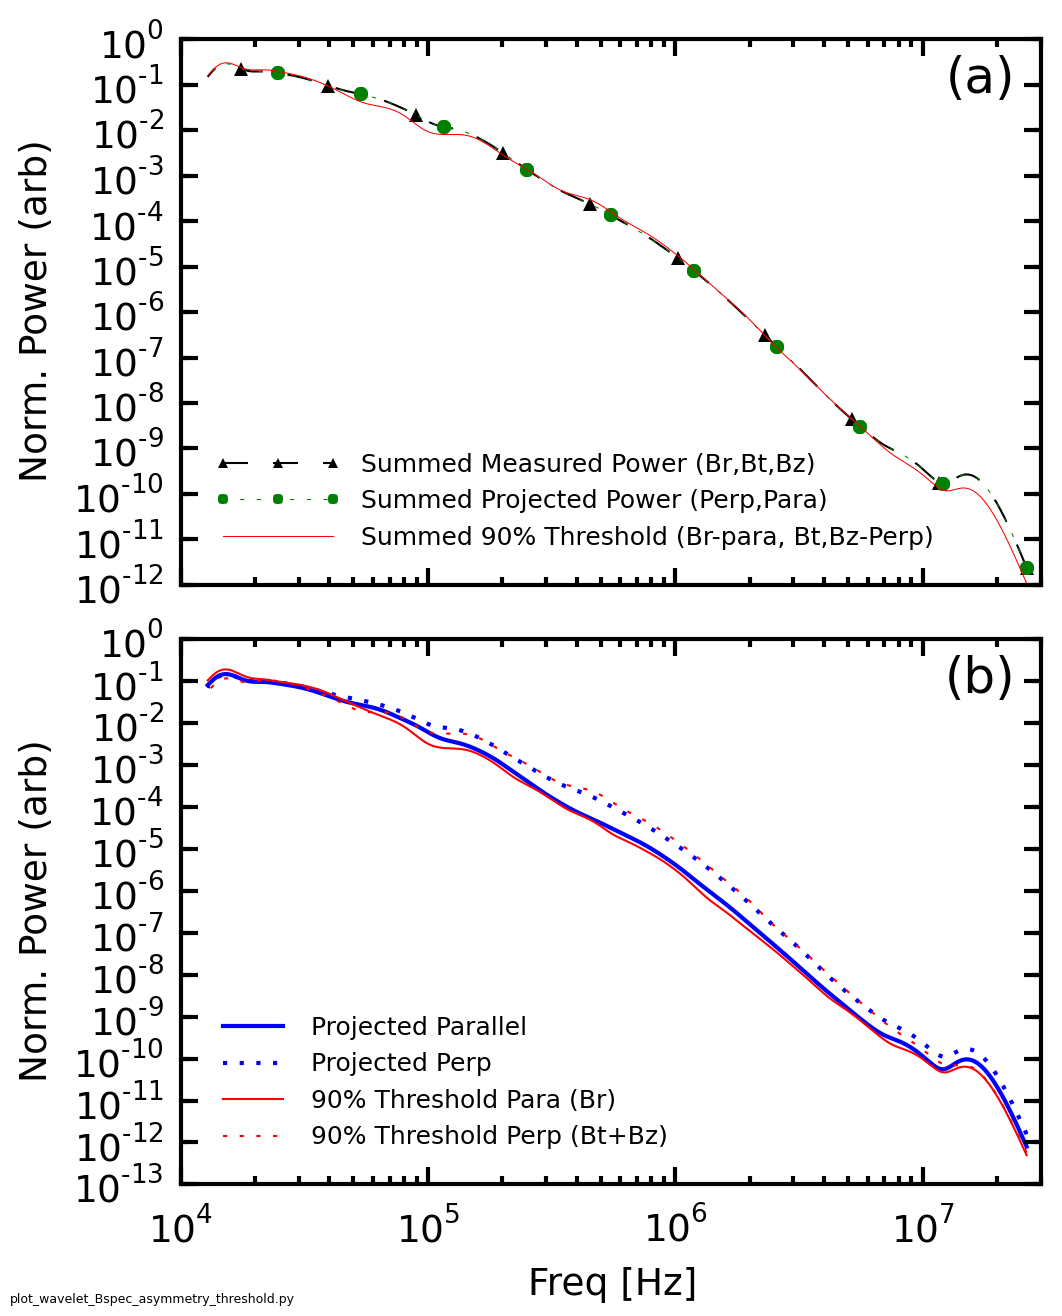
\includegraphics[width=8.5cm]{Bperppara_spectra_thresholdvsprojection40t60us}}
\caption{\label{fig:powercomparison}}
\end{figure}

As a check, the total fluctuation power spectrum is computed in three different ways and plotted in Figure~\ref{fig:powercomparison}(a) for a time range of 40 to 60$\mu s$. The total power is found by (1) summing $B_{r}(f)$, $B_{\theta}(f)$, and $B_{z}$ directly, (2) summing $B^{\parallel}(f)$ and $B^{\perp}(f)$, (3) and summing the 90\% threshold spectra of $B_{r}$, $B_{\theta}$, and $B_{z}$ from the threshold method. The curves are averaged over the total number of timesteps used in their construction so they can be directly compared amongst one another. The first two ways match exactly, showing that the total power is being properly portioned. The 90\% threshold calculation is does not match exactly, though is close. Figure~\ref{fig:powercomparison}(b) shows a comparison of the variance anistropy of the frequency power spectra as computed by the threshold and the projection methods. Again, the curves are normalized to total number of timesteps used in construction. The quantitative comparison shows that the projection method works well to compute the level of anisotropy as it compares well to the more direct, robust threshold method.

\subsection{Wavelet vs. FFT}

Figure~\ref{fig:WavevsFFT} demonstrates the correspondance between magnetic fluctuation spectra using the Wavelet analysis discussed in Section~\ref{sec:analysis} and a traditional Fast Fourier Transform. The red curves in both Fig~\ref{fig:WavevsFFT}(a) and (b) are the Wavelet generated spectra for the zero and non-zero helicity states respectively. The gray curves show a Fourier transform generated spectra for only the 40-60$\mu s$ range of each shot. Clearly, the overall shape between the two sets of curves is nearly identical. Deviations occur at low frequencies where the Wavelet transform can sample slightly lower frequencies since the analysis uses the entire time range rather than a time subset. The nature of the Wavelet transform also allows for higher resolution binning especially at these lower frequencies. The Wavelet transform, especially with the particular mother wavelet used---Morlet---tends to cause some smoothing in frequency space compared with the FFT. This is clearly seen at higher frequencies as a modes around 10MHz are more clearly observed in the FFT curver than the wavelet. However, for this particular dataset, these modes are not pertinent as they are caused by characteristics of the gun system and not by turbulence physics.

\begin{figure}[!htbp]
\centerline{
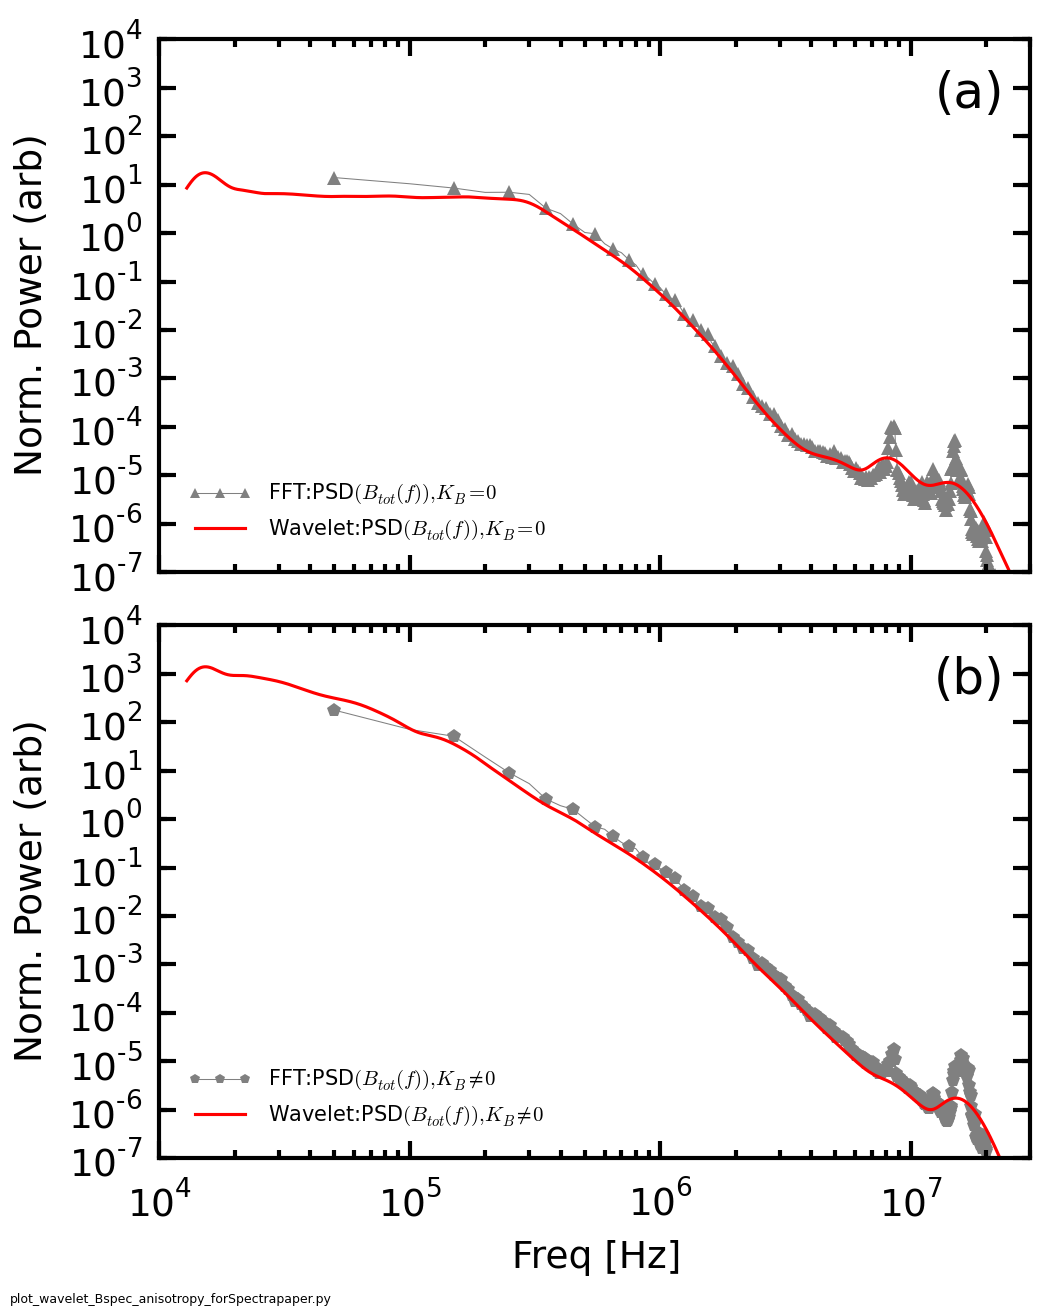
\includegraphics[width=8.5cm]{Bperppara_chan1t4_WaveletvsFFT_40t60us}}
\caption{\label{fig:WavevsFFT}}
\end{figure}

\subsection{Local vs. Global Magnetic Field}

\begin{figure}[!htbp]
\centerline{
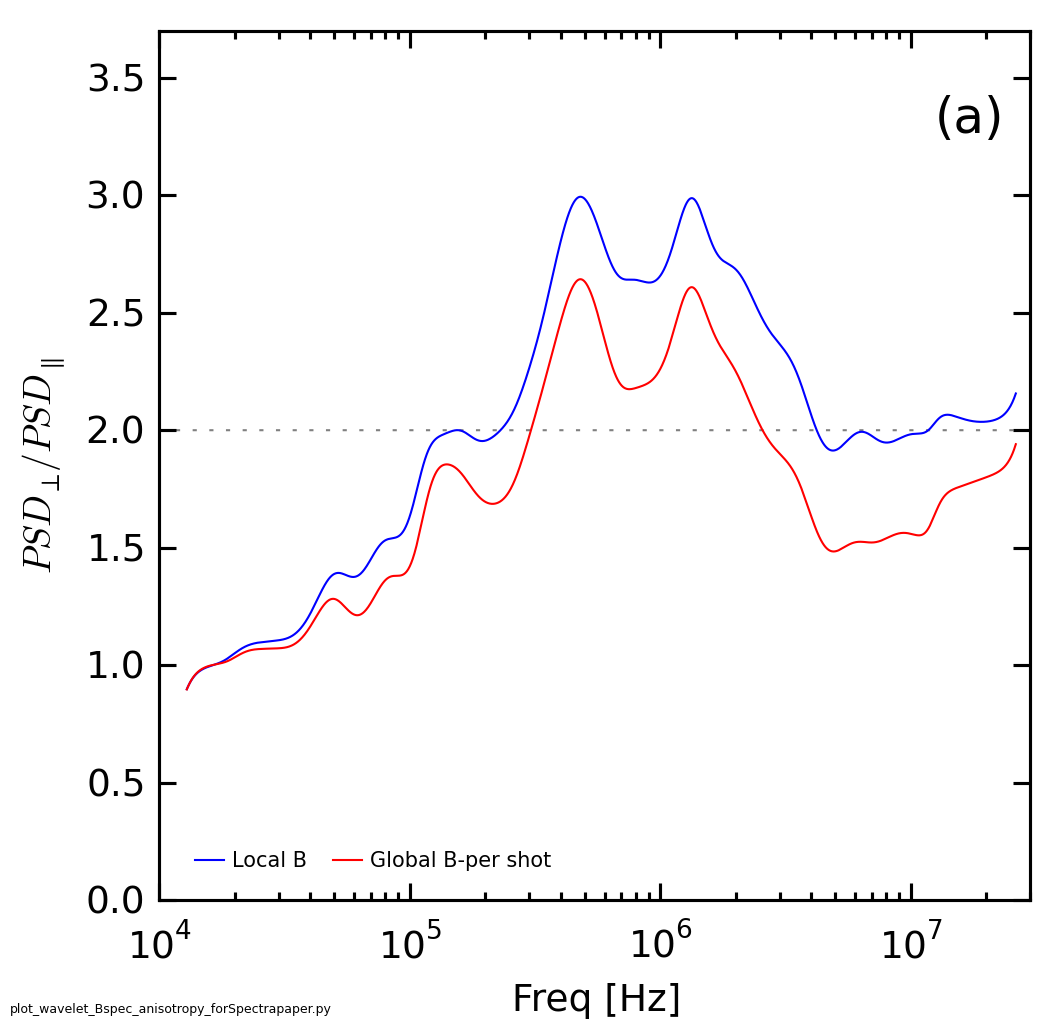
\includegraphics[width=8.5cm]{BperpparaGlobalBcomp_chan1t4_1mWbspectra}}
\caption{\label{fig:globalcomparison}}
\end{figure}

The use of a temporally local versus global magnetic field in anisotropy analysis in the solar wind has been often debated~\cite{podesta09,matthaeus12}. In this paper, a local magnetic field reference vector has been used, but a relative global field can also be used to establish anisotropy. Since the experimental data is extracted on a shot-by-shot basis, the global field in this case is the mean field for the time duration of each shot. Figure~\ref{fig:globalcomparison} shows the anisotropy ratio for local field (reference vector at each timestep) and global field (mean field for each shot). While the local field yields a ratio that is slightly higher than for the global, the trend as a function of frequency is clearly similar. This comparison can be extended to the FFT analysis which typically would not be useful for a variance analysis technique because it does not have the time resolution that the Wavelet transform does. However, since the magnetic field does not change to quickly in these plasmas, a mean field can be chosen for each shot and then used to project the full FFT spectra generated for each shot. The green curve shows this ratio, which while not as distinct as the wavelet generated ratio, nevertheless shows a similar trend especially in the kHz to MHz range. These results all suggest that though the use of a global versus local field may modify the exact numerical relationship, an anisotropy trend can be observed in either case if it is present in the plasma.
% ----------------------------------------------------------------
\section*{Acknowledgements}
%  We gratefully acknowledge many useful discussions with William Matthaeus. This work has been funded by the US DoE Experimental Plasma Research program and the National Science Foundation.  The simulations were performed using the advanced computing resources (Cray XC30 Edison system) at the National Energy Research Scientific Computing Center.
% ----------------------------------------------------------------
\section*{References}
\begin{thebibliography}{99}

\bibitem{goldstein95} M.L. Goldstein, D.A. Roberts, and W.H. Matthaeus. Magnetohydrodynamic Turbulence in the Solar Wind. Annu. Rev. Astron. Astrophys. {\bf 33} 283-325 (1995).

\bibitem{tumarsch95} C.-Y. Tu and E. Marsch. MHD Structures, Waves and Turbulence in the Solar Wind: Observations and Theories. Space Sci. Rev. {\bf 73} 1-210 (1995).

\bibitem{podesta07} J.J. Podesta, D.A. Roberts, and M.L. Goldstein. Spectral Exponents of Kinetic and Magnetic Energy Spectra in Solar Wind Turbulence. ApJ. {\bf 664} 543-548 (2007).

\bibitem{alexandrova09} O. Alexandrova, J. Saur, C. Lacombe, A. Mangeney, J. Mitchell, S.J. Schwartz, and P. Robert. Universality of Solar Wind Turbulent Spectrum from MHD to Electron Scales. Phys. Rev. Lett. {\bf 103} 165003 (2009).

\bibitem{sahraoui09} F. Sahraoui, M.L. Goldstein, P. Robert and Yu. V. Khotyaintsev. Evidence of a Cascade and Dissipation of Solar-Wind Turbulence at the Electron Gyroscale. Phys. Rev. Lett. {\bf 102} 231102 (2009).

\bibitem{horbury12} T.S. Horbury, R.T. Wicks, C.H.K. Chen. Anisotropy in Space Plasma Turbulence: Solar Wind Observations. Space Sci Rev. {\bf 172} 325-342 (2012).

\bibitem{harmon05} J.K. Harmon and W.A. Coles. Modeling radio scattering and scintillation observations of the inner solar wind using oblique Alfven/ion cyclotron waves. J. Geophys. Res. {\bf 110} A03101 (2005).

\bibitem{howes12a} G.G. Howes, D.J. Drake, K.D. Nielson, T.A. Carter, C.A. Kletzing and F. Skiff. Toward Astrophysical Turbulence in the Laboratory. Phys. Rev. Lett. {\bf 109} 255001 (2012).

\bibitem{ren11} Y. Ren, A.F. Almagri, G. Fiksel, S.C. Prager, J.S. Sarff and P.W. Terry. Experimental Observation of Anisotropic Magnetic Turbulence in a Reversed Field Pinch Plasma. Phys. Rev. Lett. {\bf 107} 195002 (2011).

\bibitem{schaffner14a} D.A. Schaffner {\it et al.} Turbulence analysis of an experimental flux rope plasma. {\bf 56} 064003 (2014).

\bibitem{schaffner14b} D.A. Schaffner {\it et al.} Observation of turbulent intermittency scaling with magnetic helicity in an MHD plasma wind-tunnel. Submitted to PRL? Feb 2014.

\bibitem{kiyani13} K.H. Kiyani, S.C. Chapman, F. Sahraoui, B. Hnat, O. Fauvarque, and Yu.V. Khotyainsev. Enhanced Magnetic Compressibility and Isotropic Scale Invariance at Sub-Ion Larmor Scales in Solar Wind Turbulence. ApJ. {\bf 763} 10 (2013).

\bibitem{clauset09}A. Clauset, C. Rohilla Shalizi, M.E.J. Newman, Power-law distributions in empirical data, SIAM Rev. {\bf 51}, 661703 (2009).

\bibitem{tenbarge12} J.M. TenBarge, J.J. Podesta, K.G. Klein and G.G. Howes. Interpreting Magnetic Variance Anisotropy Measurements in the Solar Wind. ApJ. {\bf 753} 107 (2012).

\bibitem{roberts10}D. Aaron Roberts. Evolution of the spectrum of solar wind velocity fluctuations from 0.3 to 5 AU. JGR. {\bf 115}, A12 (2010).

\bibitem{podesta09}J.J. Podesta. Dependence of Solar-Wind Power Spectra on the Direction of the Local Mean Magnetic Field. ApJ. {\bf 698}, 986-999 (2009).

\bibitem{matthaeus12}W.H. Matthaeus, S. Servidio, P. Dmitruk, V. Carbone, S. Oughton, M. Wan and K.T. Osman. Local Anisotropy, Higher Order Statistics and Turbulence Spectra. ApJ. {\bf 750}, 103 (2012).

\bibitem{torrence98}C. Torrence, G.P. Compo, A practical guide to wavelet analysis. Bull. Am. Meteorol. Soc. {\bf 79}, 6178 (1998).

%\bibitem{Belmabrouk98} Belmabrouk, H., and M. Michard (1998), Taylor length scale measurement by laser Doppler velocimetry, Exp. Fluids, 25, 69Ð76.

%\bibitem{Matthaeus05} Matthaeus, W. H. and Dasso, S. and Weygand, J. M. and Milano, L. J. and Smith, C. W. and Kivelson, M. G., Phys. Rev. Lett. 95, 231101 (2005) Spatial Correlation of Solar-Wind Turbulence from Two-Point Measurements

%\bibitem{Weygand07} Weygand, J. M., Matthaeus, W. H., Dasso, S., Kivelson, M. G., and Walker, R. J. (2007), J. Geophys. Res., 112, A10201.

%\bibitem{Weygand09} Weygand, J. M., Matthaeus, W. H., Dasso, S., Kivelson, M. G., Kristler, L. M., and Mouikis, C. (2009), J. Geophys. Res., 114, A07213.

%\bibitem{Weygand10} Weygand, J. M., Matthaeus, W. H., El-Alaoui, M., Dasso, S., and Kivelson, M. G. (2010), J. Geophys. Res., textit115, A12250.

%\bibitem{Weygand11} Weygand, J. M., Matthaeus, W. H., Dasso, S., and Kivelson, M.G. (2011), J. Geophys. Res., 116, A08120.

%\bibitem{Matthaeus08} Matthaeus W. H., Weygand, J. M., Chuychai, P., Dasso, S., Smith, C. W., and Kivelson, M. (2008), Astrophys. J., 678, L141.

%\bibitem{frisch95}Frisch, U. 1995, {\it Turbulence} (Cambridge: Cambridge Univ. Press)

%\bibitem{sorrisovalvo99}Sorriso-Valvo, L. {\it et al.} Geophys. Res. Lett. {\bf 26}, 1801–1804 (1999).

%\bibitem{wan12}Wan, M. {\it et al.} ApJ. {\bf 744} 177 (2012).

%\bibitem{sorrisovalvo01}Sorriso-Valvo, L. {\it et al.} Planet. Space Sci. {\bf 49}, 1193–1200 (2001).

%\bibitem{marrelli05}Marrelli, L. {\it et al.} Phys. Plasmas. {\bf 12}, 030701 (2005).

%\bibitem{Greco08}A. Greco, P. Chuychai, W. H. Matthaeus, S. Servidio and P. Dmitruk, Intermittent MHD structures and classical discontinuities, Geophys. Res. Lett. {\bf 35}, L19111 (2008).

%\bibitem{Greco09}Greco, A., Matthaeus, W. H., Servidio, S., Chuychai, P., and Dmitruk, P.: Statistical Analysis of Discontinuities in Solar Wind ACE Data and Comparison with Intermittent MHD Turbulence, ApJ {\bf 691}, L111 (2009).

%\bibitem{Wan09}Wan, M., Oughton, S., Servidio, S., and Matthaeus, W. H.: Generation of non-Gaussian statistics and coherent structures in ideal magnetohydrodynamics, Phys. Plasmas {\bf 16}, 080703 (2009).

%\bibitem{Servidio11b}Servidio, S. {\it et al}, J. Geophys. Res. {\bf 116}, A09102 (2011).

%\bibitem{Gray13} T. Gray, M. R. Brown, and D. Dandurand. Phys. Rev. Lett. {\bf 110}, 085002 (2013). 



%\bibitem{Taylor86} J. B. Taylor, Rev. Mod. Phys. {\bf 58}, 741 (1986).

%\bibitem{Matthaeus80} W.H. Matthaeus and D. Montgomery, Ann. N.Y. Acad. Sci. {\bf 357}, 203 (1980).





%\bibitem{wan12}M. Wan, K. T. Osman, W. H. Matthaeus, and S. Oughton, Investigation of intermittency in magnetohydrodynamics and solar wind turbulence: scale-dependent kurtosis, ApJ {\bf 744}, 171 (2012).

%\bibitem{Gray10}T. Gray, V. S. Lukin, M. R. Brown, C. D. Cothran, Three-dimensional reconnection and relaxation of merging spheromak plasmas, Phys. Plasmas {\bf 17}, 102106 (2010).

%\bibitem{goldstein94}Goldstein, M.L., Roberts, D.A. and Fitch, C.A. Jour. Geo. Res. {\bf 99} 11519-11538 (1994).

%\bibitem{ji95}Ji, H., Prager, S.C. and Sarff, J.S. Phys. Rev. Lett. {\bf 74} 2945 (1995).

%\bibitem{telloni12}Telloini, D. {\it et al.}. ApJ. {\bf 751} 19 (2012).

%\bibitem{matthaeusVelli11}Matthaeus, W.H. and Velli, M. Space Sci. Rev. {\bf 160} 145-168 (2011).

%\bibitem{greco12}A. Greco {\it et al.} ApJ. {\bf 749} 105 (2012).

\end{thebibliography}

\end{document}

